\documentclass[useAMS,usenatbib]{mn2e}

\usepackage{times}
\usepackage{graphicx}
\usepackage{amsmath}
\usepackage{amssymb}
\usepackage{color}
\usepackage{journal_names}
\usepackage{paralist}
\usepackage[inline]{enumitem}

\newcommand{\kms}{\mbox{\,km~s$^{-1}$}}
\setlength{\tabcolsep}{0.06in}   % reduce the column spacing in the Tables
 
\title[The Fornax Cluster VLT Spectroscopic Survey]{The Fornax Cluster VLT Spectroscopic Survey. I -- Spectroscopy and compilation of the globular cluster catalogue in the cluster core}

\author[Pota et al.]{\noindent
Vincenzo Pota et al. $^{1}$\thanks{E-mail: vincenzo.pota@gmail.com}, 
%Nicola R. Napolitano$^{1}$, 
%Michael Hilker$^{3}$, 
%Massimo Capaccioli$^{2}$, 
%\and Enrica Iodice$^{1}$, 
%Marilena Spavone$^{1}$, 
%Christine Schulz,
%Thomas Puzia$^{5}$,
%Robert Munoza$^{5}$,
%\and Maurizio Paolillo$^{5}$,
%Raffaele D'abrusco$^{5}$,
%Lino Grado$^{5}$ $NRN: era nel proposal? non mi sembra che è tra i destinatari del draft, lo puoi anche togliere...
%Pietro Schipani$^{5}$ $NRN Pietro va aggiunto
\\~\\
$^1$ INAF -- Osservatorio Astronomico di Capodimonte, Salita Moiariello, 16, 80131 - Napoli, Italy\\
%$^5$ Australian Astronomical Observatory, PO Box 915, North Ryde, NSW 1670, Australia\\
}

\voffset=-0.6in
\begin{document}

\label{firstpage}

\maketitle
\begin{abstract}
We present the results of a wide spectroscopic survey aimed at detecting extragalactic globular clusters (GCs) in the core of the Fornax cluster. This program is part of the Fornax Cluster VLT Spectroscopic Survey (FVSS) aimed at gathering kinematical information of stars and compact sources in the Fornax Core using different VLT instruments, in synergy with the Fornax Deep Survey carried out at the VLT Survey Telescope (VST). GC candidates were selected in multi-band VST and VISTA images. About 4500 low resolution spectra (from 4800 to 10000\AA) were observed in 25 VLT/VIMOS masks covering the central 1 deg$^2$ around the dominant galaxy NGC~1399 corresponding to $\sim$200 kpc. We describe the methodology used for data reduction and data analysis. We found a total of 387 unique physical objects (372 GCs and 15 ultra compact dwarfs) in the field covered by our observation. Most of these objects are overlapped and possibly associated with NGC~1399, with only 10\% likely associated with other giant galaxies. However the kinematics of the objects beyond 10 arcmin (i.e. $\sim$60 kpc) is consistent with the one of an unblund population and likely dominated by intracluster globular clusters. The new dataset is complementary to the many GC catalogues already present in the literature and it brings the total number of tracer particles around  NGC~1399 to more than 1130 objects. This is a valuable reference for the study of the galaxy cluster environment and for the dynamics and kinematics of giant galaxies out to the intracluster regions corresponding to about $1/4$ of the cluster virial radius, which will be mapped with unprecedented details. Here we have found that the velocity dipersion of the GC population (whether or not this is split in red and blue populations) show the signature at around $R\sim10’$ of a kinematical transition from a low $v_{\rm rms}$ regime to a higher one, with the former being consistent with the central velocity dispersion of NGC 1399 (the central cluster galaxy) and the latter being consistent with the velocity dispersion of the cluster galaxies. This demonstrates that at $R>10’$ both GC populations feel strongly the cluster potential, rather than the more fable galaxy potential. These kinematical evidences corroborate the photometric evidence found in the deep galaxy photometry of a transition radius between the bright central galaxy and the outer exponential halo and show, from the dynamical point of view, the emergence of an intracluster population of GCs in the Fornax Cluster.

\end{abstract}

\begin{keywords}
galaxies:star clusters -- galaxies:evolution-- galaxies: kinematics and dynamics
\end{keywords}

\section{Introduction}

Nearby galaxy clusters are ideal laboratories for studying the evolution of low- and high mass galaxies as well as dense stellar systems (globular clusters, compact dwarf galaxies, etc.) in dense environments. The Virgo and Fornax clusters are closest galaxy clusters, hence providing privileged target where detailed observations fn the galaxy and small stellar system content can be performed and unique test bench to test galaxy formation theories. 

The Fornax cluster is the most massive galaxy structure after the Virgo cluster within 20 Mpc and it is an ideal target to study the effect of the environment on the structure and assembly of galaxies of any type, from the massive central giant early-type systems to the dwarf galaxies. Despite its regular appearance, it has been found that the assembly of the Fornax cluster is still ongoing. Although its core seems in an evolved phase (Grillmair et al. 1994; Jord an et al. 2007) and most of the bright ($m_B < $  15 mag) cluster members are early-type galaxies (Ferguson 1989), the presence of stellar and GC tidal streams (e.g. Iodice et al. 2016, D’Abrusco et al. 2016, Eisenhardt et al. 2017) have revealed that there are still signs of active galaxy interactions in the region inside 200 kpc, which mirrors the large scale activity, including the accretion of the Fornax-A (NGC 1316) subgroup into the cluster core along a cosmic web filament (Drinkwater et al. 2001; Scharf et al. 2005).

The Fornax Deep Survey\footnote{ESO programme ID (094.B-0687)} (FDS) is a joint project based on Guaranteed Time Observation surveys, FOCUS (P.I. R. Peletier) and VEGAS (P.I. E. Iodice, Capaccioli et al. 2015), aimed to study the formation and assembly of the Fornax Cluster out to its virial radius with a variety of observations. These include
deep photometry, supplemented by cross-match with other wavelength observations such as  X-rays (e.g. Paolillo et al. 2002) and multi-object and integral-field spectroscopy.
The cornerstone of FDS is deep multiband ($u$, $g$, $r$ and $i$) imaging data from the OmegaCam (Kuijken 2011) camera at the VLT Survey Telescope (VST, Schipani et al. 2012), covering an area of $\sim30$ $deg^2$ of the cluster out to the virial radius. The area includes the Fornax-A subgroups, hence providing a full coverage of the cluster structure under assembly.  The depth of the imaging dataset reaches $\sim 30$ mag/arcsec$^2$ in the $g$-band (see Iodice et al. 2016, 2017), among the deepest acquired on the cluster so far (Venhola et al. 2018). VISTA/VIRCAM observations in $J$ and $K$ ($Ks$ = 23.4 $AB$ mag, and $J = 23.4$ $AB$ mag) are also available (see e.g. Munoz et al. 2015), to complement the optical data and optimise galaxy and globular cluster membership and the selection of follow-up targets (e.g. globular clusters, GCs hereafter, and/or ultra compact dwarf galaxies, UCDs hereafter). 

The multi-band deep images have been used to study the light distribution and colours of cluster galaxies out to 8-10 effective radii and beyond to characterise the faint galaxy haloes. These studies revealed the presence of ultra-faint stellar structures in the core of Fornax: fingerprints of past and ongoing interaction between galaxies falling into the deep potential well of the cluster (Iodice et al. 2016, Venhola et al. 2017). The same conclusion is backed up by the complex distribution of globular clusters in the Fornax cluster (D’Abrusco et al. 2016, Cantiello et al. 2017).

To kinematically map the complexity of the cluster core out to at least 200 kpc using discrete kinematical tracers (e.g. GCs and UCDs) and finally connect the large scale kinematics down to the scale of the dwarf galaxies, we have started a multi-instrument observational effort called the Fornax Cluster VLT Spectroscopic Survey (FVSS). As a part of this effort we have acquired integral field spectroscopy of dwarfs galaxies (see Mentz et al. 2016, Spiniello et al. in preparation), a counter dispersed imaging run with FORS2 to detect and measure radial velocities of planetary nebulae (Spiniello et al. 2018, submitted as FVSS II) and multi-object spectroscopy of GC and UCD candidates with VIMOS/VLT.

The latter program is the topic of this paper, where we present the radial velocity catalogue of GCs and UDGs in the core of Fornax, which is complementary to archival spectroscopic GC datasets of the Fornax cluster: Schuberth et al. (2010a) (which incorporates the catalogue of Dirsch et al. 2004), Bergond et al. (2007) and other catalogues discussed throughout the text. The novelty of the sample discussed in this paper is the uniform coverage of the central 1 deg$^2$ of the Fornax core which will allow us to provide a spatially complete map of the kinematics of the galaxies in the field out to the regions where they meet the intracluster field (see e.g., Napolitano et al. 2003; Arnaboldi et al. 2012). Here, dynamical times are longer than the central galaxy regions and we expect to find the kinematical signature of the substructures already seen in the FDS photometry (Iodice et al. 2016) or other gravitational interactions such as shells and tidal tails in the kinematics of the galaxy outskirts or intracluster regions (Napolitano et al. 2002, 2003; Murante et al. 2007; Bullock & Johnston 2005; Rudick, Mihos,and McBride 2006; Duc et al. 2011; Longobardi et al. 2015a,b). FVSS, in synergy with FDS, will be the foundation of a multifaceted project to constrain the baryonic and dark mass distribution in the core of the Fornax cluster with high precision, thus shedding light on the assembly history of massive galaxies in one of the nearest dense environments.

In this first paper of the series, we present the radial velocity catalogue of GCs. 
%There are also planetary nebula datasets around NGC 1399 (Napolitano et al. 2002, McMillan et al. 2010) and NGC 1316 (McMillan et al. 2012) that provide an extension of the stellar kinematics out to several effective radii and overlapping with the area covered by our analysis, which we will use to compare the average properties of the velocity field of the galaxy core.
The assumed distance is 19.95 Mpc (Tonry et al. 2010).
%NRN: Aaron suggests to use Blakeslee+09 which has D=20.0 Mpc. I thing we can keep Tonry   

The paper is structured as follows: Section \ref{sec:data} describes the data acquisition and reduction. The redshift estimation is discussed in Section \ref{sec:zest}, results are presented in Section \ref{sec:analysis} and discussed in \ref{sec:discussion}. We summarise the results of the paper and conclude in Section \ref{sec:conclusions}. 

\section{Data}
\label{sec:data}

This Section discusses all the steps undertaken to compile the spectroscopic catalogue discussed in this paper. The 
workflow consists of selecting a sample of GC candidates based on photometric selection criteria (\S 
\ref{sec:selectionGC}) and then using the derived sample to design multi-object masks (\S \ref{sec:VIMOSpointings}) for follow-up 
observations (\S \ref{sec:observations}).

\begin{figure*}
\centering
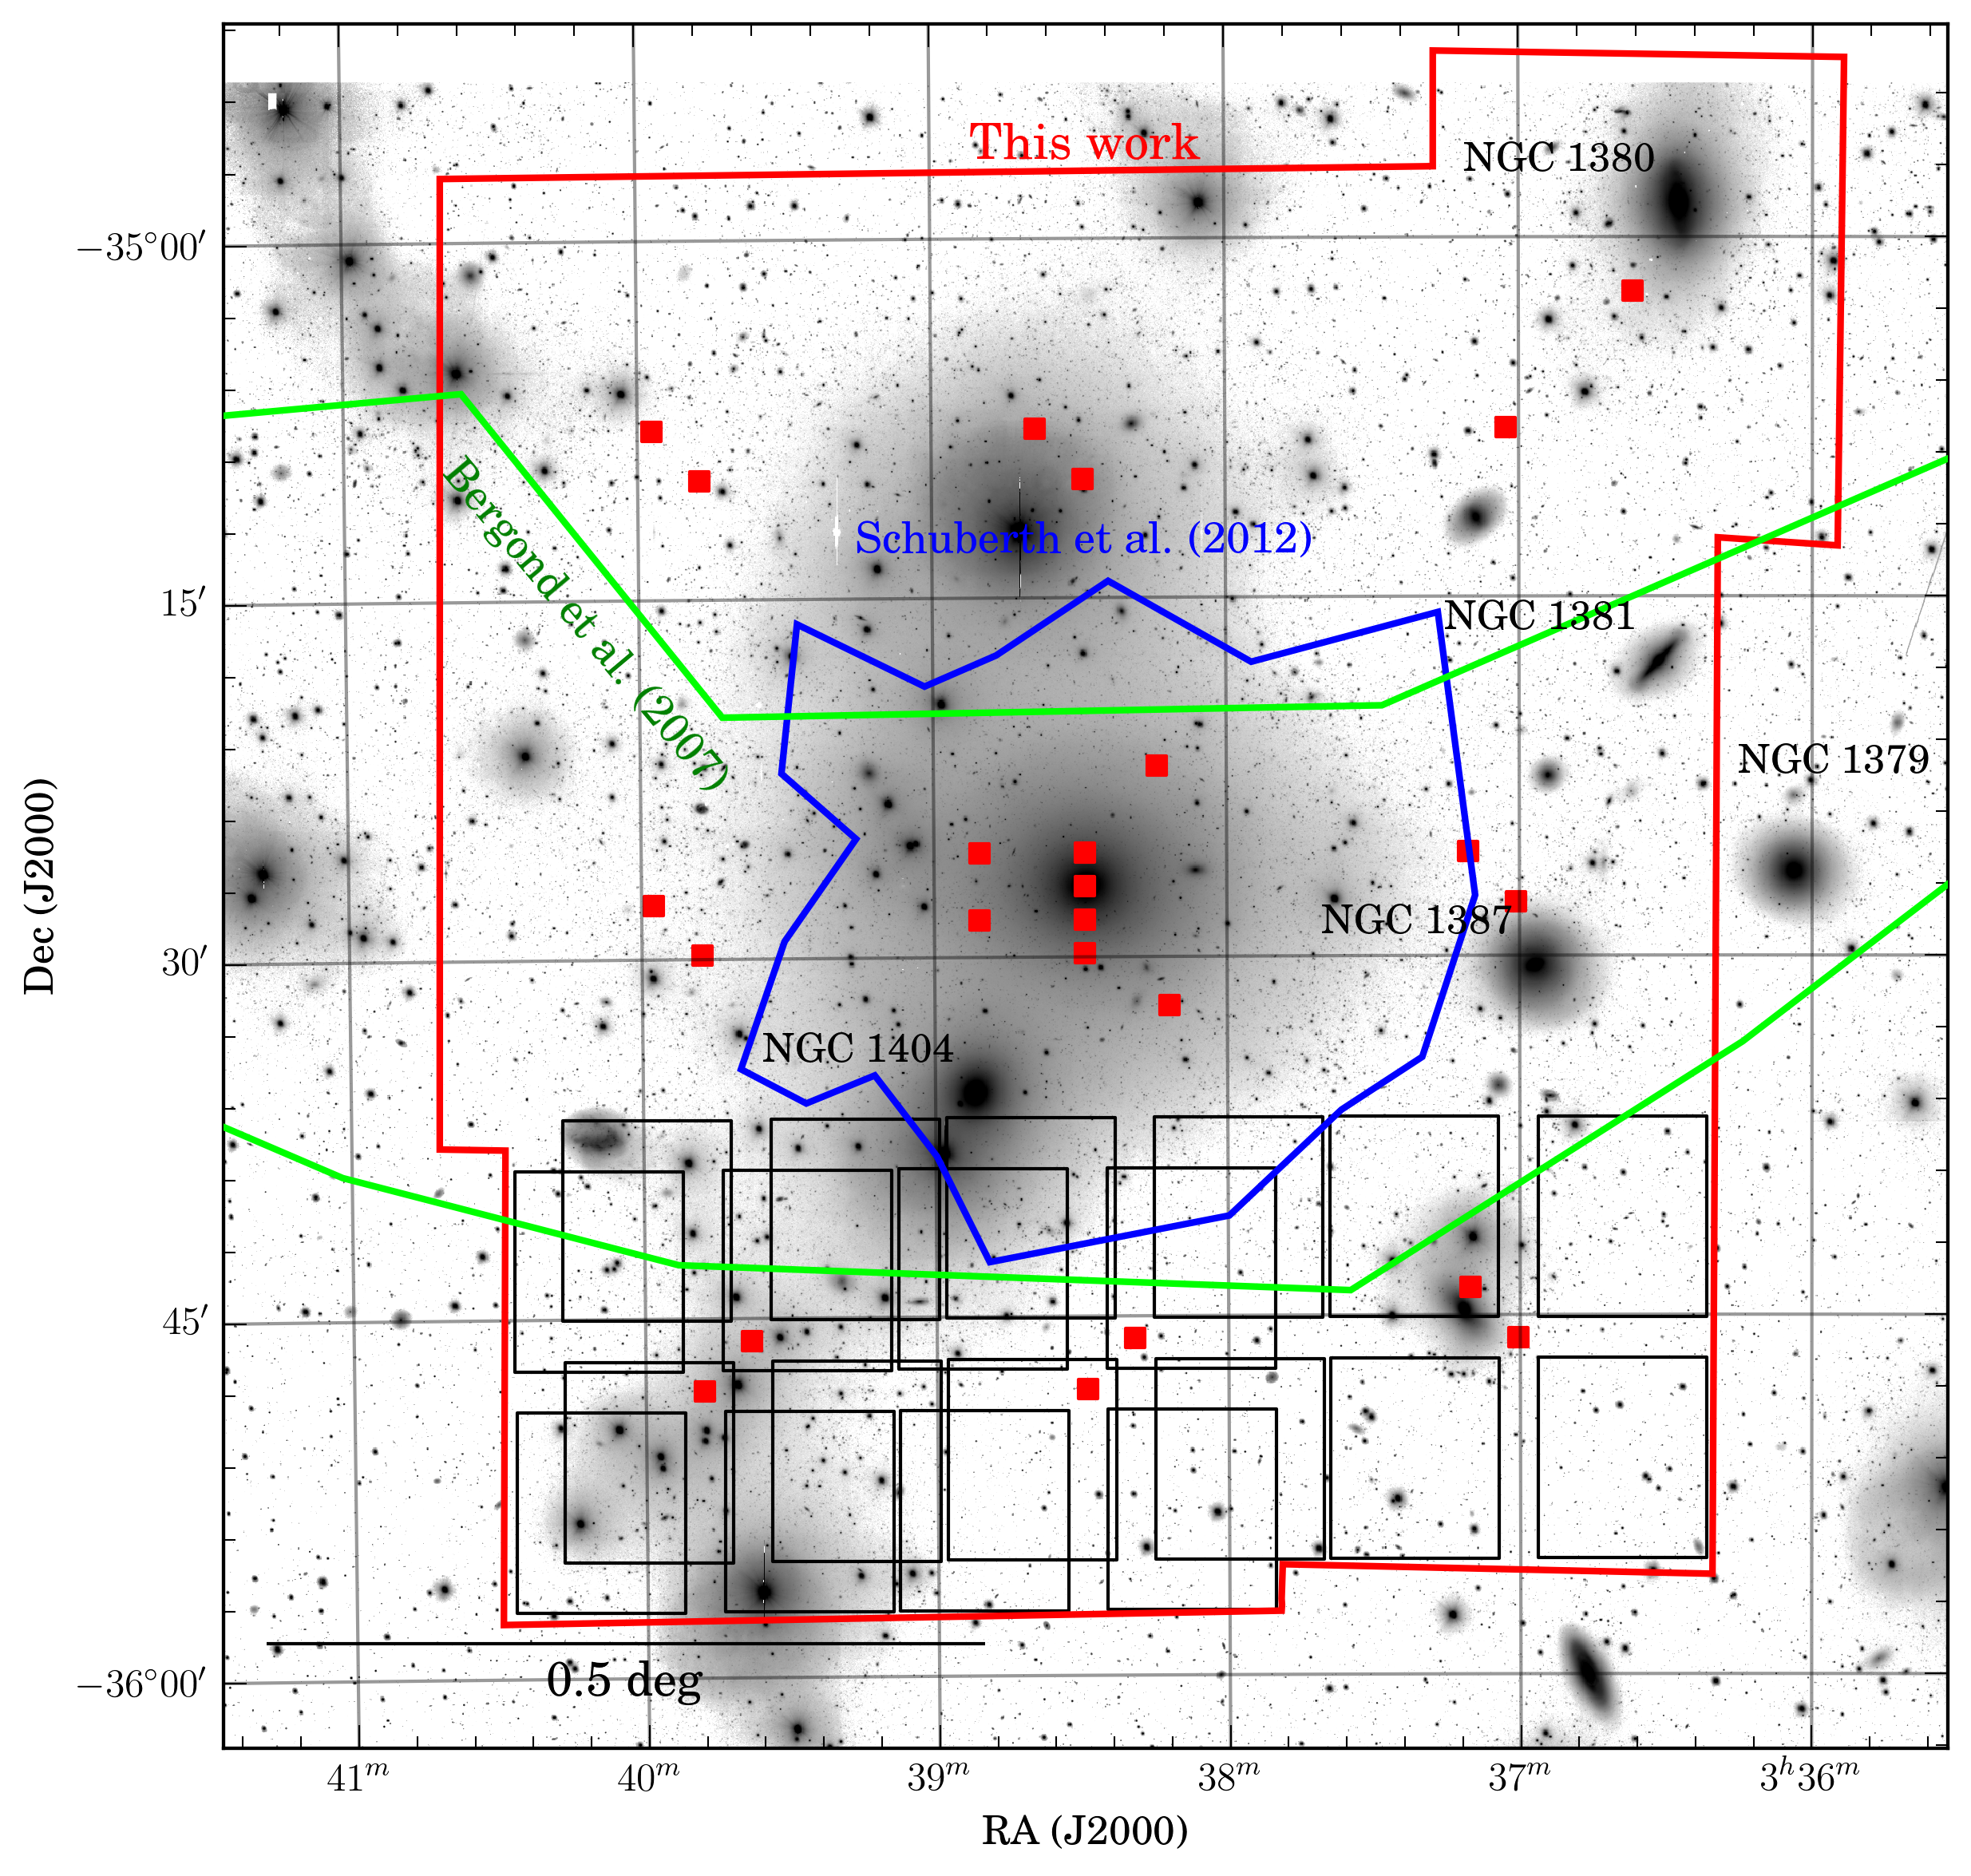
\includegraphics[scale=0.7]{figures/fov.png} 
\caption{Layout of the observations. The background image is a mosaic of several VST/OmegaCAM pointings in the $g$-
band. The central galaxy is NGC~1399. Additional Fornax galaxies are also labeled. The red boxes mark the centers of all 
25 VIMOS pointings. The footprints of some VIMOS masks are shown on the bottom for illustrative purposes. Note how 
the VIMOS masks are intertwined to maximize spatial coverage. The region covered by all 25 VIMOS is outlined in red, 
whereas the regions covered by literature studies are shown in green \citep{Bergond07} and blue \citep{Schuberth}}.
%NRN: Aaron: Schuberth in the figure is 2010 not 2012 
\label{fig:fov}
\end{figure*}

\subsection{Selection of globular cluster candidates}
\label{sec:selectionGC}
The selection of GC candidates was based on VST/OmegaCAM photometry in the $g$ and $i$ band from the FDS survey 
\citep{DAbrusco16,Iodice16} and preliminary VISTA/VIRCAM photometry in the $K_s$ band from the NGFS (Next 
Generation Fornax Survey, \citealt{Munoz14}). 
In the combined 2-colour $giK_s$ diagram, spectroscopically confirmed GCs from \citet{Schuberth} are confined to a restricted colour-
colour space. %NRN: Aaron suggests to include a figure: I think we can skip this and show in case the referee laso asks. However, if this figure is available we can consider to add it now.
We defined a polygon around the radial velocity--members, which serves as the prime selection criterion for our GC candidates. 

As an additional criterion we used the published wide-field Washington photometry from \citet{Dirsch04} and \citet{Bassino} to construct a $C-i$ vs. $i-K_s$ diagram. Since the Washington $C$-band is similar to a $u$-band filter and the $uiK_s$ plane is a very powerful tool to discriminate GCs from foreground and background objects \citep{Munoz14}, the $CiK_s$ plane is the cleanest selection criterion. Unfortunately, the spatial coverage of the Washington photometry is not complete in the central square degree due to chip gaps and the restricted field-of-view. Out of the 1065 unique spectroscopic targets with $CiK_s$ photometry, 809 (or $\sim$76\%) are within this selection polygon.

Of the 4340 unique spectroscopic targets (see Sect. 2.2) 4321 have $giK_s$ photometry, and 2643 (or $\sim$ 61 \%) of those are confined to the selection polygon. 
Here, we applied a magnitude restriction of 17.0$<i<$23.0 mag to our GC candidate sample in order to avoid severe contamination by foreground stars on the bright side and too low signal-to-noise spectra on the faint side. 
%The magnitude distribution of the above mentioned 4321 unique spectroscopic targets can be seen in the $(g-i)$ vs. $i$ CMD of FigureXX (fnxgtocmdgiKadp.pdf).
For the very central regions of NGC~1399, which are dominated by the galaxy light, we found additional GC candidates taking advantage on the more accurate photometry and morphological classification derived from {\it Hubbe Space Telescope}/ACS data by \citet{Puzia14}.

Finally, all other allocated fibers, i.e. the remaining 1678 slits, besides a small portion used to dupicate targets, were split to observe known stars and background galaxies. These latter will be discussed in a separate paper. 

The FDS $gi$, the NGFS $K_s$, Washington $C$ as well as the central ACS  photometric catalogs were matched with SExtractor photometry of point and extended sources in all pre-images (ESO programme 094.B-0687(A)), which were taken in $R$-band prior to the spectroscopic observations. The x and y coordinates of sources in the pre-images are needed to create VIMOS catalogs for the creation of mask files with the VMMPS (VIMOS Mask Preparation Software,\citealt{Bottini05}) from ESO.

\subsection{VIMOS pointings and mask design}
\label{sec:VIMOSpointings}

A total of 25 VIMOS masks were designed covering the central square degree around NGC~1399. The masks were interleaved in such a way that the gaps between the four VIMOS CCDs (or quadrants) were covered by the adjacent mask. 

In Figure \ref{fig:fov} we show the spatial distribution of the VIMOS pointings, along with the footprints of archival observations in the same sky region from \citet{Schuberth} and \citet{Bergond07}. It is clear that the mask distribution is much more homogeneous with respect to previous studies, although our target sampling varies across the field. The total covered area also contains other giant galaxies, namely, NGC~1404, NGC~1387 and NGC~1380.  
Figure \ref{fig:2dsplit} shows how the 2-dimensional density of allocated slits is considerably higher in the center with respect to the outskirts. Eight of the 25 pointings were dedicated to the central 25$\times$25 arcmin to account for the higher density of GC candidates close toNGC~1399. 

The use of the MR grism allows a multiplexing of two in wavelength direction (parallel to declination), i.e. spectra are not overlapping if slits are placed close to the bottom and top of the chip areas in all quadrants. 
For a first automatic slit allocation we used VMMPS with a catalog of GC candidates from the $giK_s$ selection as input. Since the result of the automatic slit allocation was not satisfactory, we optimized the slit allocation of targets manually, for example by de-centering some targets in the slits while still keeping enough sky, or by allowing some overlap in wavelength range for multiplexed spectra, and by giving preference to targets that also fulfill the $CiK_s$ selection criterion. The remaining free area on the chips was then filled with slits centered on GC candidates from the $(g-i)$ colour selection or on pre-selected background galaxies to allow ancillary science on photometric redshift confirmations.

In this way, we defined 4574 slits in total for the 25 pointings ranging form 157 to 202 slits per pointing (or 36 to 60 slits per quadrant). Several slits were positioned in such a way to cover more than one target if they had the same declination and a small distance in right ascension (of the order of 10$''$ or less {\bf MN comment, check this nubber with Michael}). Since the fields are overlapping, about 300 targets have been observed twice and four targets even three times through different masks. This allows us to evaluate the systematic uncertainties of the radial velocity measurements and correct for them between different masks. Discounting all duplications, we ended up with about 4340 unique targets
for which spectra were taken. 

%Those are shown as red dots in FigureXX (fnxgtocooadp.pdf) together with confirmed GC candidates from previous  radial velocity measurements (blue circles). Our targets and confirmed  members are also shown with the same symbols in the 2-colour diagrams of the $giK_s$ (FigureXX, fnxgto2colgiKadp.pdf) and $CiK_s$ (FigureXX, fnxgto2colCiKadp.pdf) planes and the corresponding $(g-i)$ vs. $i$ (FigureXX, fnxgtocmdgiKadp.pdf) and $(C-i)$ vs. $i$ (FigureXX, fnxgtocmdCiKadp.pdf) CMDs.

\begin{figure}
\centering
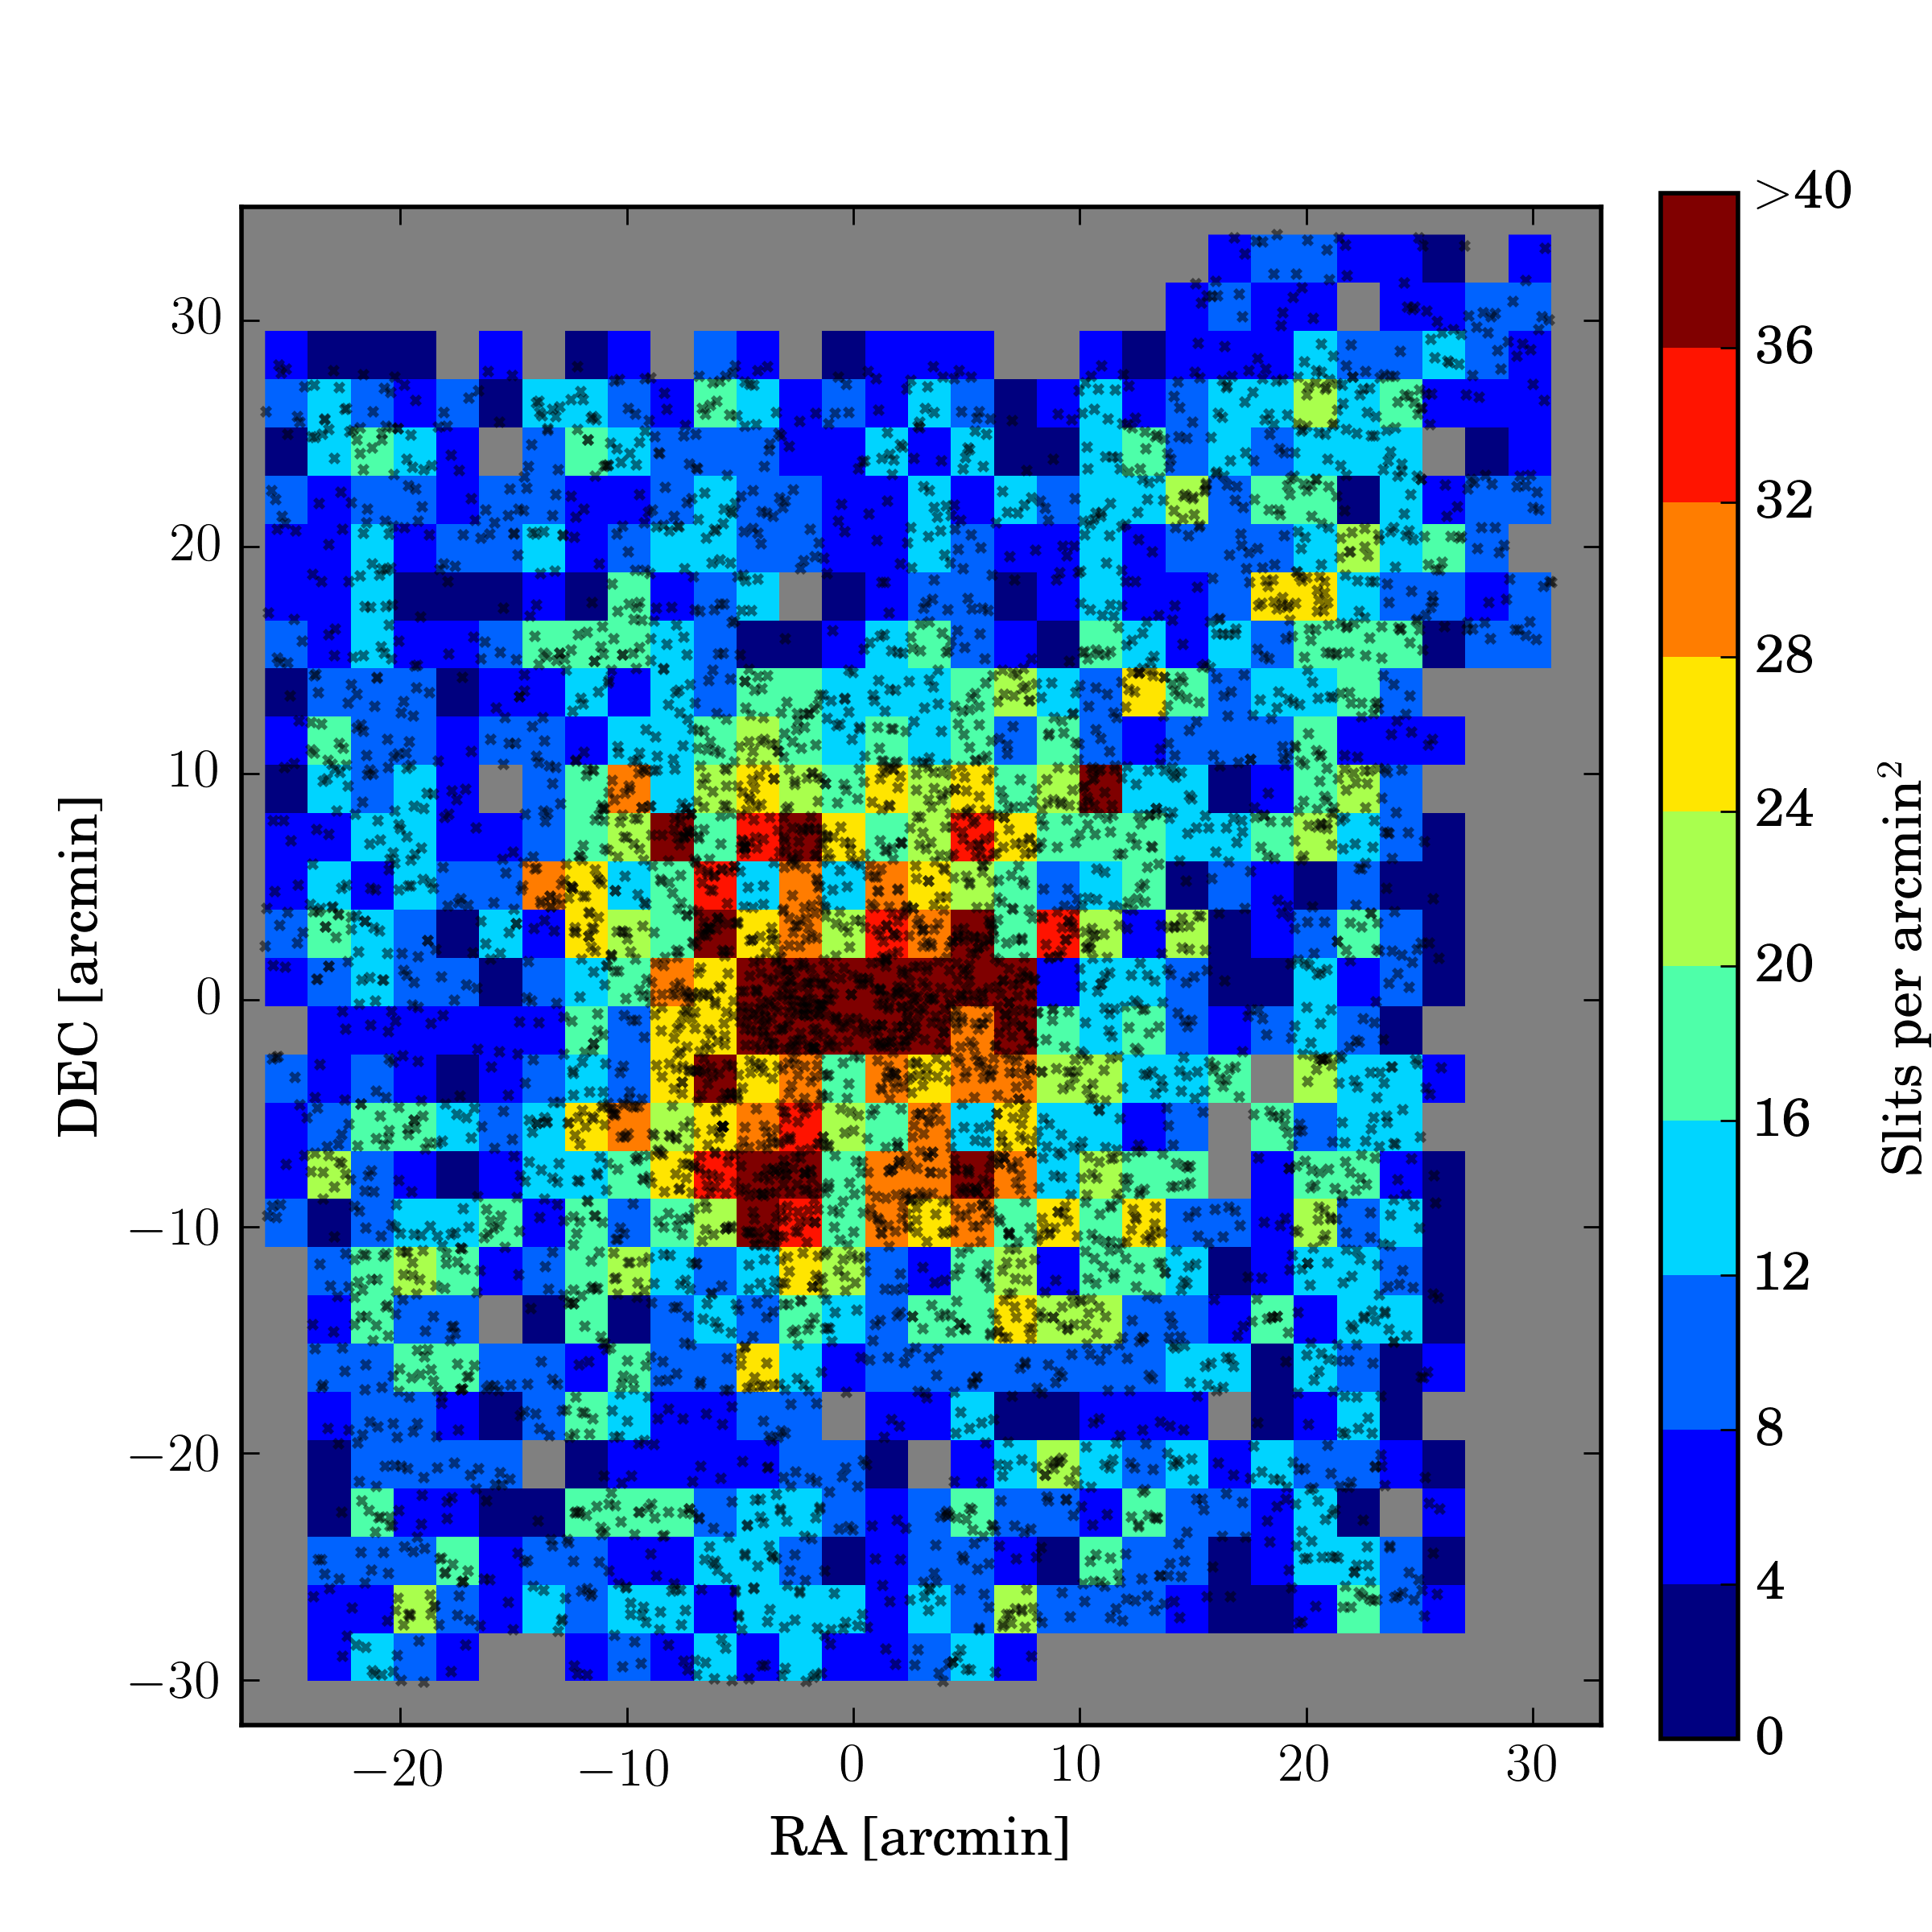
\includegraphics[width=\columnwidth]{figures/slitdist.png} 
\caption{Two dimensional spatial density of VIMOS slits. Slits are shown as small black crosses, whereas the colours represent total counts in boxes of $2\times2$ arcmin$^2$. Axes express the distance in arcmin from NGC~1399. More slits were placed towards the center of the cluster, where the target density is higher. North is toward the top, East to the left.}
\label{fig:2dsplit}
\end{figure}

\subsection{Observations}
\label{sec:observations}

Spectroscopic observations were carried out with the VIsible MultiObject Spectrograph (VIMOS, \citealt{LeFevre}), mounted on the VLT-UT3 Melipal telescope at the ESO Paranal observatory in Chile and used in multi-object mode. The observations have been acquired in Period 94 (Program ID: 094.B-0687, PI: M. Capaccioli), from October 2014 to January 2015. 
The VIMOS spectrograph was equipped with a filter CG475, which cuts off wavelengths bluer than 4750 \AA\ , and a MR grating with a spectral resolution $R = 580$ (or 12.0 \AA\ FWHM) 
%NRN: Aaron asks: is it really a constant resolution with w.l.?
and a dispersion of $2.5$ \AA /~pix. All slits had a width of 1 arcsec. The pixel scale in the spatial direction was 0.205 arcsec/pix. This setup allows us to explore the spectral window ranging from $4800$ to $10000$~\AA. Sky transparency was set to clear.

VIMOS is equipped with four CCDs, arranged in four quadrants with chip gaps of $\sim$2 arcmin in vertical and horizontal direction (see examples of the VIMOS detector footprints in Figure \ref{fig:fov}). Overall, one VIMOS mask set covers a field of 4 $\times$ (7 $\times$ 8 arcmin$^2$). All masks were observed for 1.5 hours in total, divided into three dithered exposures of 30 minutes. Observations were carried out in service mode in gray-time conditions between October 2014 and January 2015. The seeing ranged from 0.66 arcsec to 1.15 arcsec, with a median of 0.85 arcsec. 

\subsection{Data reduction}

The reduction of the VIMOS data was performed using the Reflex 
environment \citep{Freudling13} of the ESO VIMOS pipeline. 
For each VIMOS mask, the data consist of four 
quadrants with three individual exposures for each quadrant, flatfields and
arc lamp calibration exposures that were taken directly after the science 
exposures. Each science exposure has a distribution of slits containing the 
science spectra of the targets contaminated by the emission spectrum of the 
earth's atmosphere. Since the wavelengths of the sky emission lines are 
precisely known they can be used for the absolute wavelength calibration of 
the spectra.

In order to obtain the final wavelength calibrated science spectra, we 
proceeded as follows. First, a wavelength calibration 
is performed using the provided arc lamp spectrum. Second, we calculated
the residual shift of the sky lines are shifted with respect to their restframe 
wavelength. For this purpose we provided our own sky line catalog, in which 
the wavelengths of prominent sky lines, in particular in the Ca triplet 
region, are listed. The pipeline determines this shift for each spectrum in 
each science exposure individually, which is essential because the wavelength 
shifts are not the same for the three exposures: the shift is largest for the 
first exposure and smallest for the third exposure ({\bf quationfrom MN: Could you give an estimate of the magnitude of the effect e.g. 0.3 to 0.1A?}). This is caused by the 
change of instrument flexure between the first science exposure and the final 
arc lamp exposure. In other words, the third science exposure is taken 
closest in time, i.e. under almost the same instrument conditions, to the arc 
lamp exposure, and thus its wavelength calibration is the most accurate one. 
Finally, the pipeline stacks the three individual science exposures and 
extracts sky subtracted object spectra from the combined science frame.

Unfortunately, it turned out that the pipeline does not apply the wavelength 
shifts to the individual spectra before the stacking, meaning that the stacked
spectra are not corrected for the residual shifts. This leads to an incorrect
absolute wavelength calibration and also to a slight line broadening in the 
stacked spectra. Even though we cannot correct for the line broadening with
the current ESO pipeline version, we found a workaround to correct for the
absolute wavelength calibration of the spectra, which is necessary for an 
accurate measurement of the radial velocities of the objects. To first order, 
it can be assumed that the median wavelength shift in the stacked spectrum is 
the same as the one derived for the second exposure. Thus, we re-reduced the 
second science exposure of all available data to determine the median 
wavelength shift in each multiplex of each mask by taking the average shift 
of all spectra in that multiplex. Then, the wavelength of each stacked 
spectrum was shifted by an amount as determined by the multiplex and the mask
in which the spectrum is located. All further analyses were carried out 
on the spectra corrected in this way.

For each mask, the REFLEX pipeline outputs multi-extension fits files which include the calibrated 2D spectra, the calibrated 1D spectra (and respective errors) and a 2D model of the sky lines. To make the dataset more manageable, we implemented a python/astropy script which copies different data structures corresponding to each slit into a multi-extension fits file. Each slit is associated to a fits file which contains: the 1D scientific spectrum, the 1D error spectrum, the sky-subtracted, wavelength-corrected 2D spectrum and a thumbnail of the object of $5\times5$ arcsec$^2$ from $g$-band VST imaging. 

\section{Redshift estimation}
\label{sec:zest}

A total of 6700 spectra were extracted by the REFLEX pipeline. This number includes the objects genuinely associated with the Fornax cluster (i.e., GCs, UDCs or dwarf galaxies), as well as Galactic stars, background galaxies and sources with signal-to-noise (S$/$N) too low to be classified with certainty. 

Radial velocities were computed with {\it iraf/fxcor}, which performs cross-correlation between the Fourier-transformed scientific spectrum and a Fourier-transformed set of template spectra \citep{Tonry79}. {\it Fxcor} was preferred to full spectra fitting approaches (e.g. pPXF, \citealt{Cappellari04}) because the former does not require initial guesses on the radial velocity and it is more CPU efficient. 

The Indo-U.S. Library of Coud\'e Feed Stellar Spectra \citep{Valdes04} was used as library of template spectra. The library contains 1273 stellar spectra, observed with a dispersion of $0.44$ \AA /pix and a resolution of $\sim 1$ \AA . The spectra cover the 3460 -- 9464 \AA\ range, which overlaps nicely with the wavelength range of our VIMOS spectra. From the whole library, we selected a random subset of 40 stars with spectral types from \textit{F} to \textit{M} because this is the range expected for metal-poor to metal-rich GCs ({\bf question from MN: What stellar type were these? Giants presumably.

Did you choose a different random set each time? Or only once which you applied to the rest of the analysis.

I worry about this approach giving poor fits for stars if you don’t happen to have enough template stars close enough to the type you are fitting.
}). 


The 40 stellar spectra were convolved with a Gaussian filter of standard deviation $\sigma = 12.0\mbox{\AA\ } / 2.355$ (where 12.0 \AA\ is the FWHM resolution of our VIMOS spectra). 

The scientific spectra were prepared as follows. First, we computed the median signal-to-noise per pixel $S/N$, where the signal $S$ is measured in the range 5000-6600 \AA\ and the noise $N$ is the noise returned by the REFLEX pipeline in the same wavelength range. Second, telluric bands in the range 6850 -- 7688 \AA\ and some troublesome skylines were replaced with the fit to the spectral continuum. The continuum was computed with iraf/continuum by averaging ten contiguous pixels and interpolating the result with a cubic spline coupled with a $3\sigma$ rejection algorithm.  

Naively, one may think that cross-convolving the full wavelength range of our VIMOS spectra will return more robust radial velocities because the number of atomic lines used for the convolution is larger. Instead, we found that using the whole wavelength range can increase uncertainties due to severe template mismatches, likely due to the low ($S/N = 12$) average $S/N$ of our spectra. Therefore, we chose to run {\it fxcor} on the region surrounding the Calcium Triplet (CaT) at 8498-8548-8662 \AA , because these three lines occupy a very narrow wavelength range. Therefore, we correlate the scientific spectra between 8485-8750 \AA\ with the template spectra between 8450-8720 \AA . This means that we are able to measure the radial velocities of unresolved objects between $-500 \kms$ and $+3000\kms$, which include both Galactic stars and Fornax objects.   

During the fxc{\it fxcor}or run, and prior to the correlation with the template spectra, the Fourier-transformed scientific spectra were filtered with a ramp filter. The filter was set up to cut off noisy high frequencies as well as low frequencies which may result from poor continuum fitting. The continuum was fitted with a cubic spline function.
We ran {\it fxcor} in non-interactive mode, meaning that {\it fxcor} always returns the velocity corresponding to the highest cross-correlation with the template spectrum. The final radial velocity is the median of the single radial velocities obtained from the cross-correlation with the 40 template stars. %Although this choice spared us the manual check of $6700 \times 40 = 2.6 \times 10^5$ spectra, it also increased the likelihood of template mismatch. 
To overcome extreme template mismatch (i.e. the case in which the fitted radial velocity varies considerably depending on the adopted template), we used a median-absolute-deviation algorithm (MAD) to flag radial velocities deviating more than 5$\sigma$ from the median of the radial velocities obtained from the 40 template stars. Outliers, if any, are removed from the velocity set and the final radial velocity and error are computed from the remaining measurements. 90 per cent of GCs and stars have between 0 to 5 outliers, suggesting that the effect of extreme template mismatch is small. 

The scatter in radial velocity due to normal template mismatch (i.e. due to intrinsic mixture of stellar populations in GCs) varies between 3 -- 10 \kms (after removing outliers) depending on the $S/N$ of the spectrum. The final error on the radial velocity is the median velocity error returned by {\it fxcor} summed in quadrature to the scatter due to normal template mismatch. 

\begin{figure}
\centering
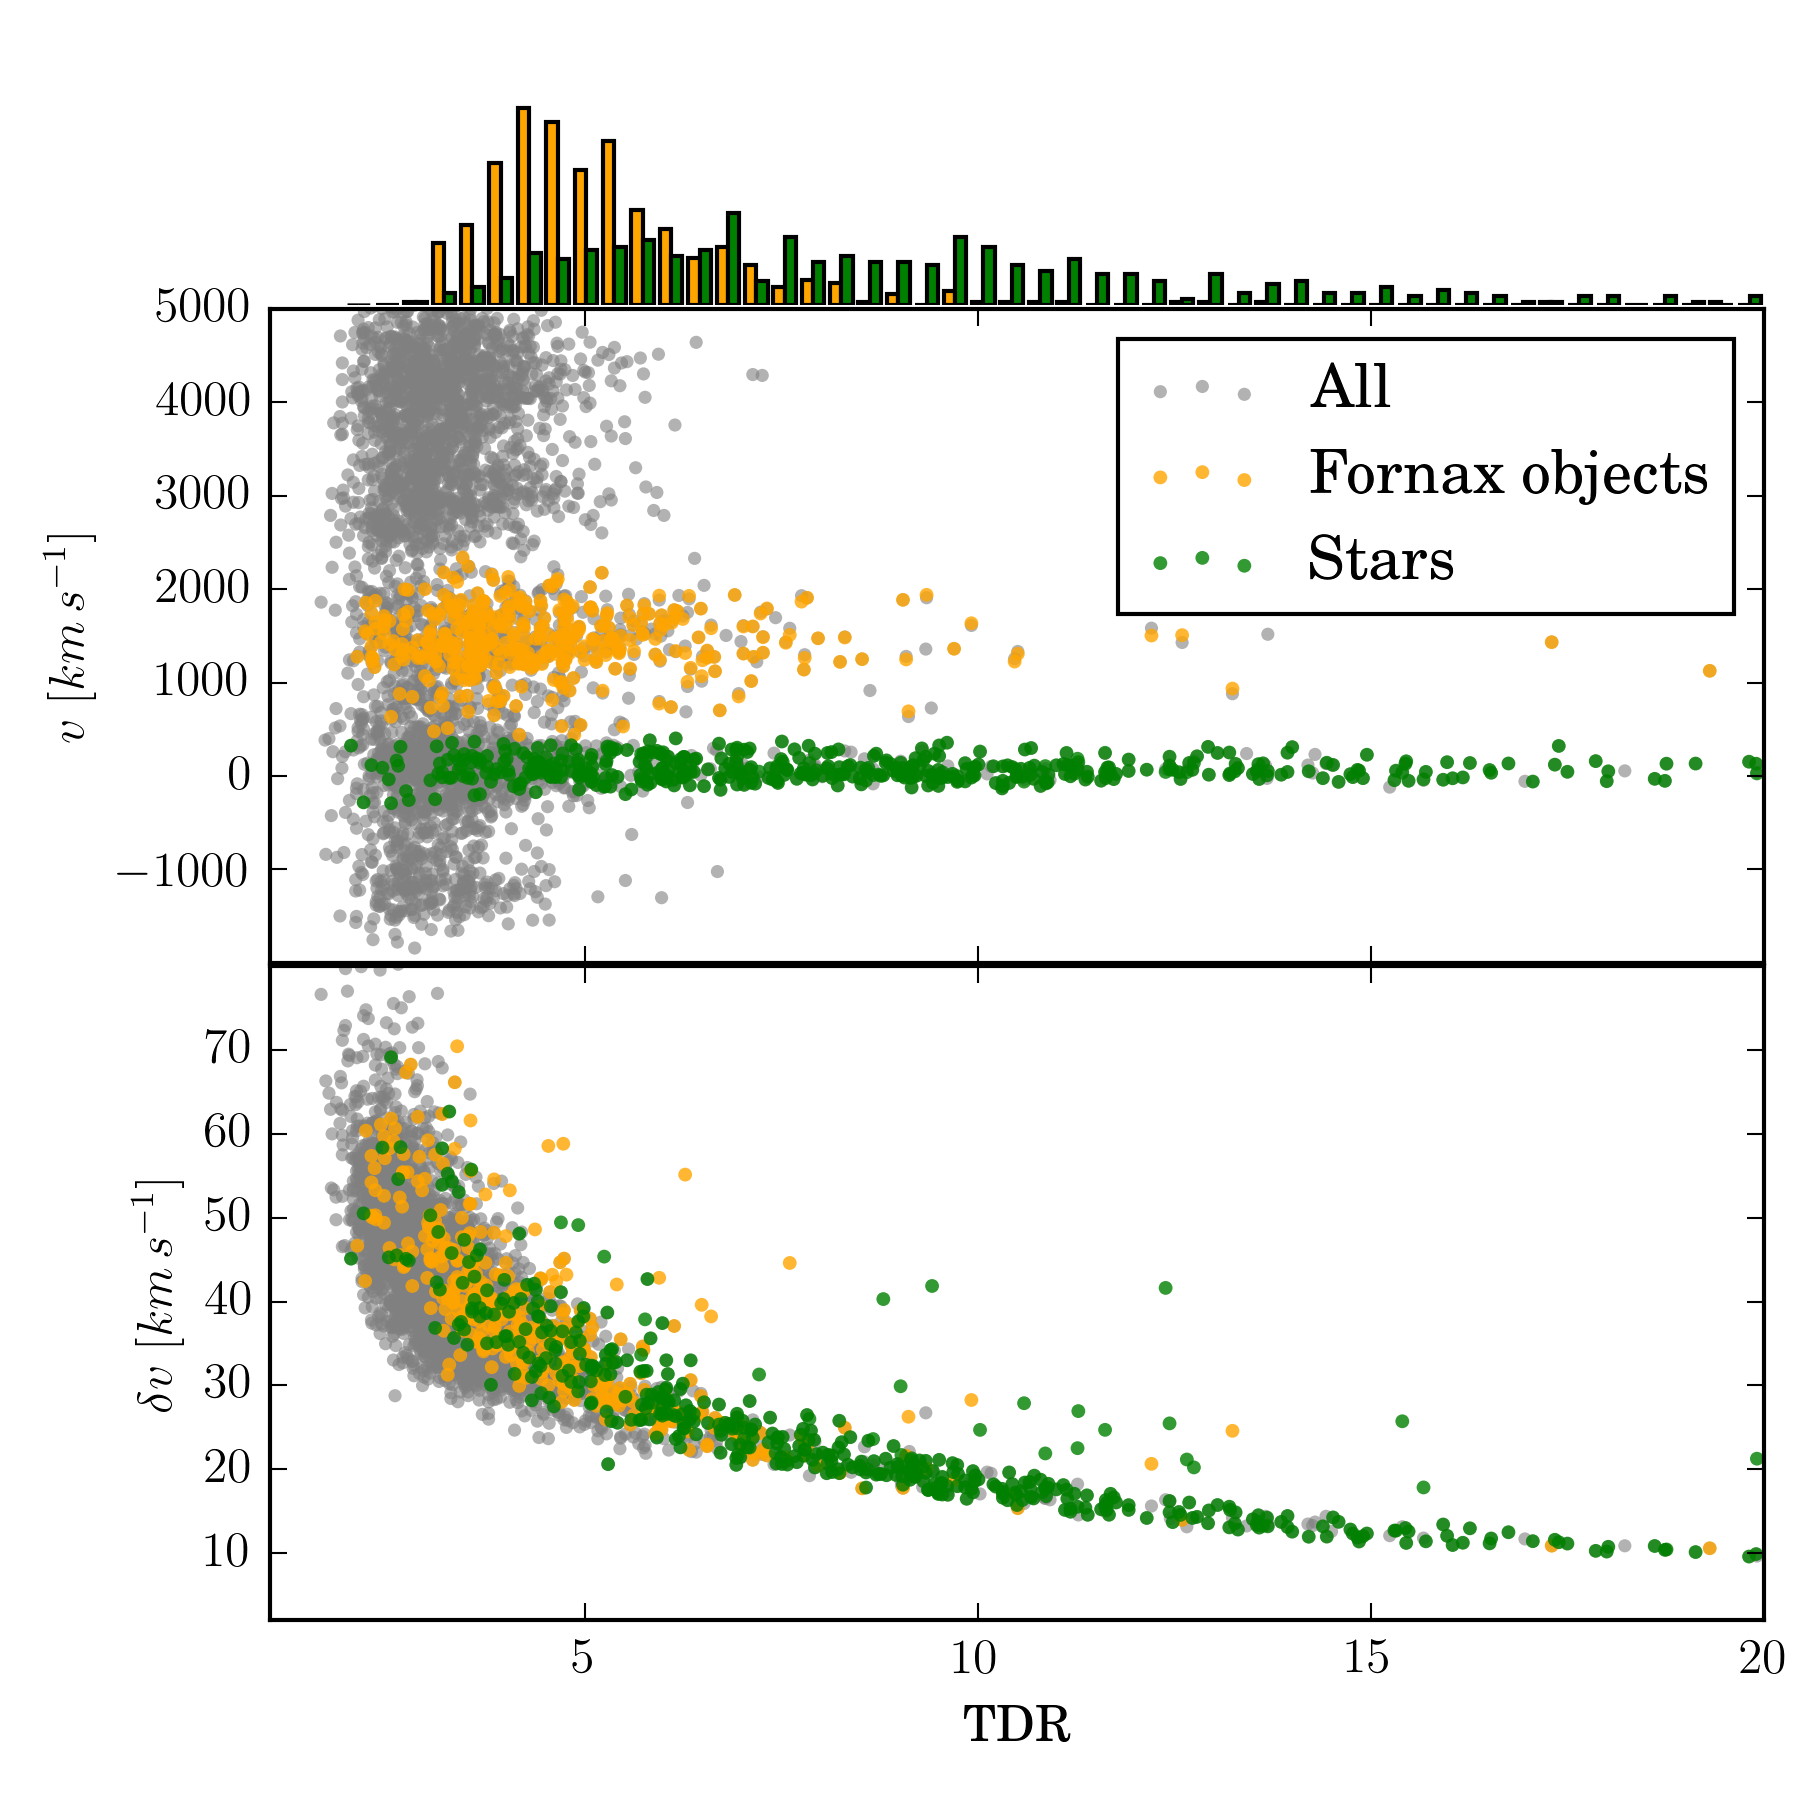
\includegraphics[width=\columnwidth]{figures/fxcor_subplot.png} 
\caption{Results from {\it iraf/fxcor} for $\sim$ 4200 spectra. The x-axis represents the Tonry \& Davies R parameter (TDR) which is a proxy for the goodness of the cross-correlation between the scientific and the template spectra. Smaller TDR corresponds to larger velocity uncertainties $\delta v$ (bottom panel) and therefore to a poorer spectral fit. The measured radial velocity $v$ is shown on the y-axis of the top panel. The sequence of objects at $v\approx 0 \kms$ are Galactic stars, whereas the cluster at $v\approx1700\kms$ are GC candidates in the Fornax cluster. The histogram on the top shows raw counts for stars and Fornax objects only, respectively. }
%NRN: question from Aaron: why are there objects with velocities like stars and like Fornax but neither green nor orange? NR: I guess that most of them are because they have not been validated in the eye inspection. I understand this for the low TDR, but fr the higher TDR? Are these spectra with issues? 
\label{fig:tdr}
\end{figure}

\begin{figure}
\centering
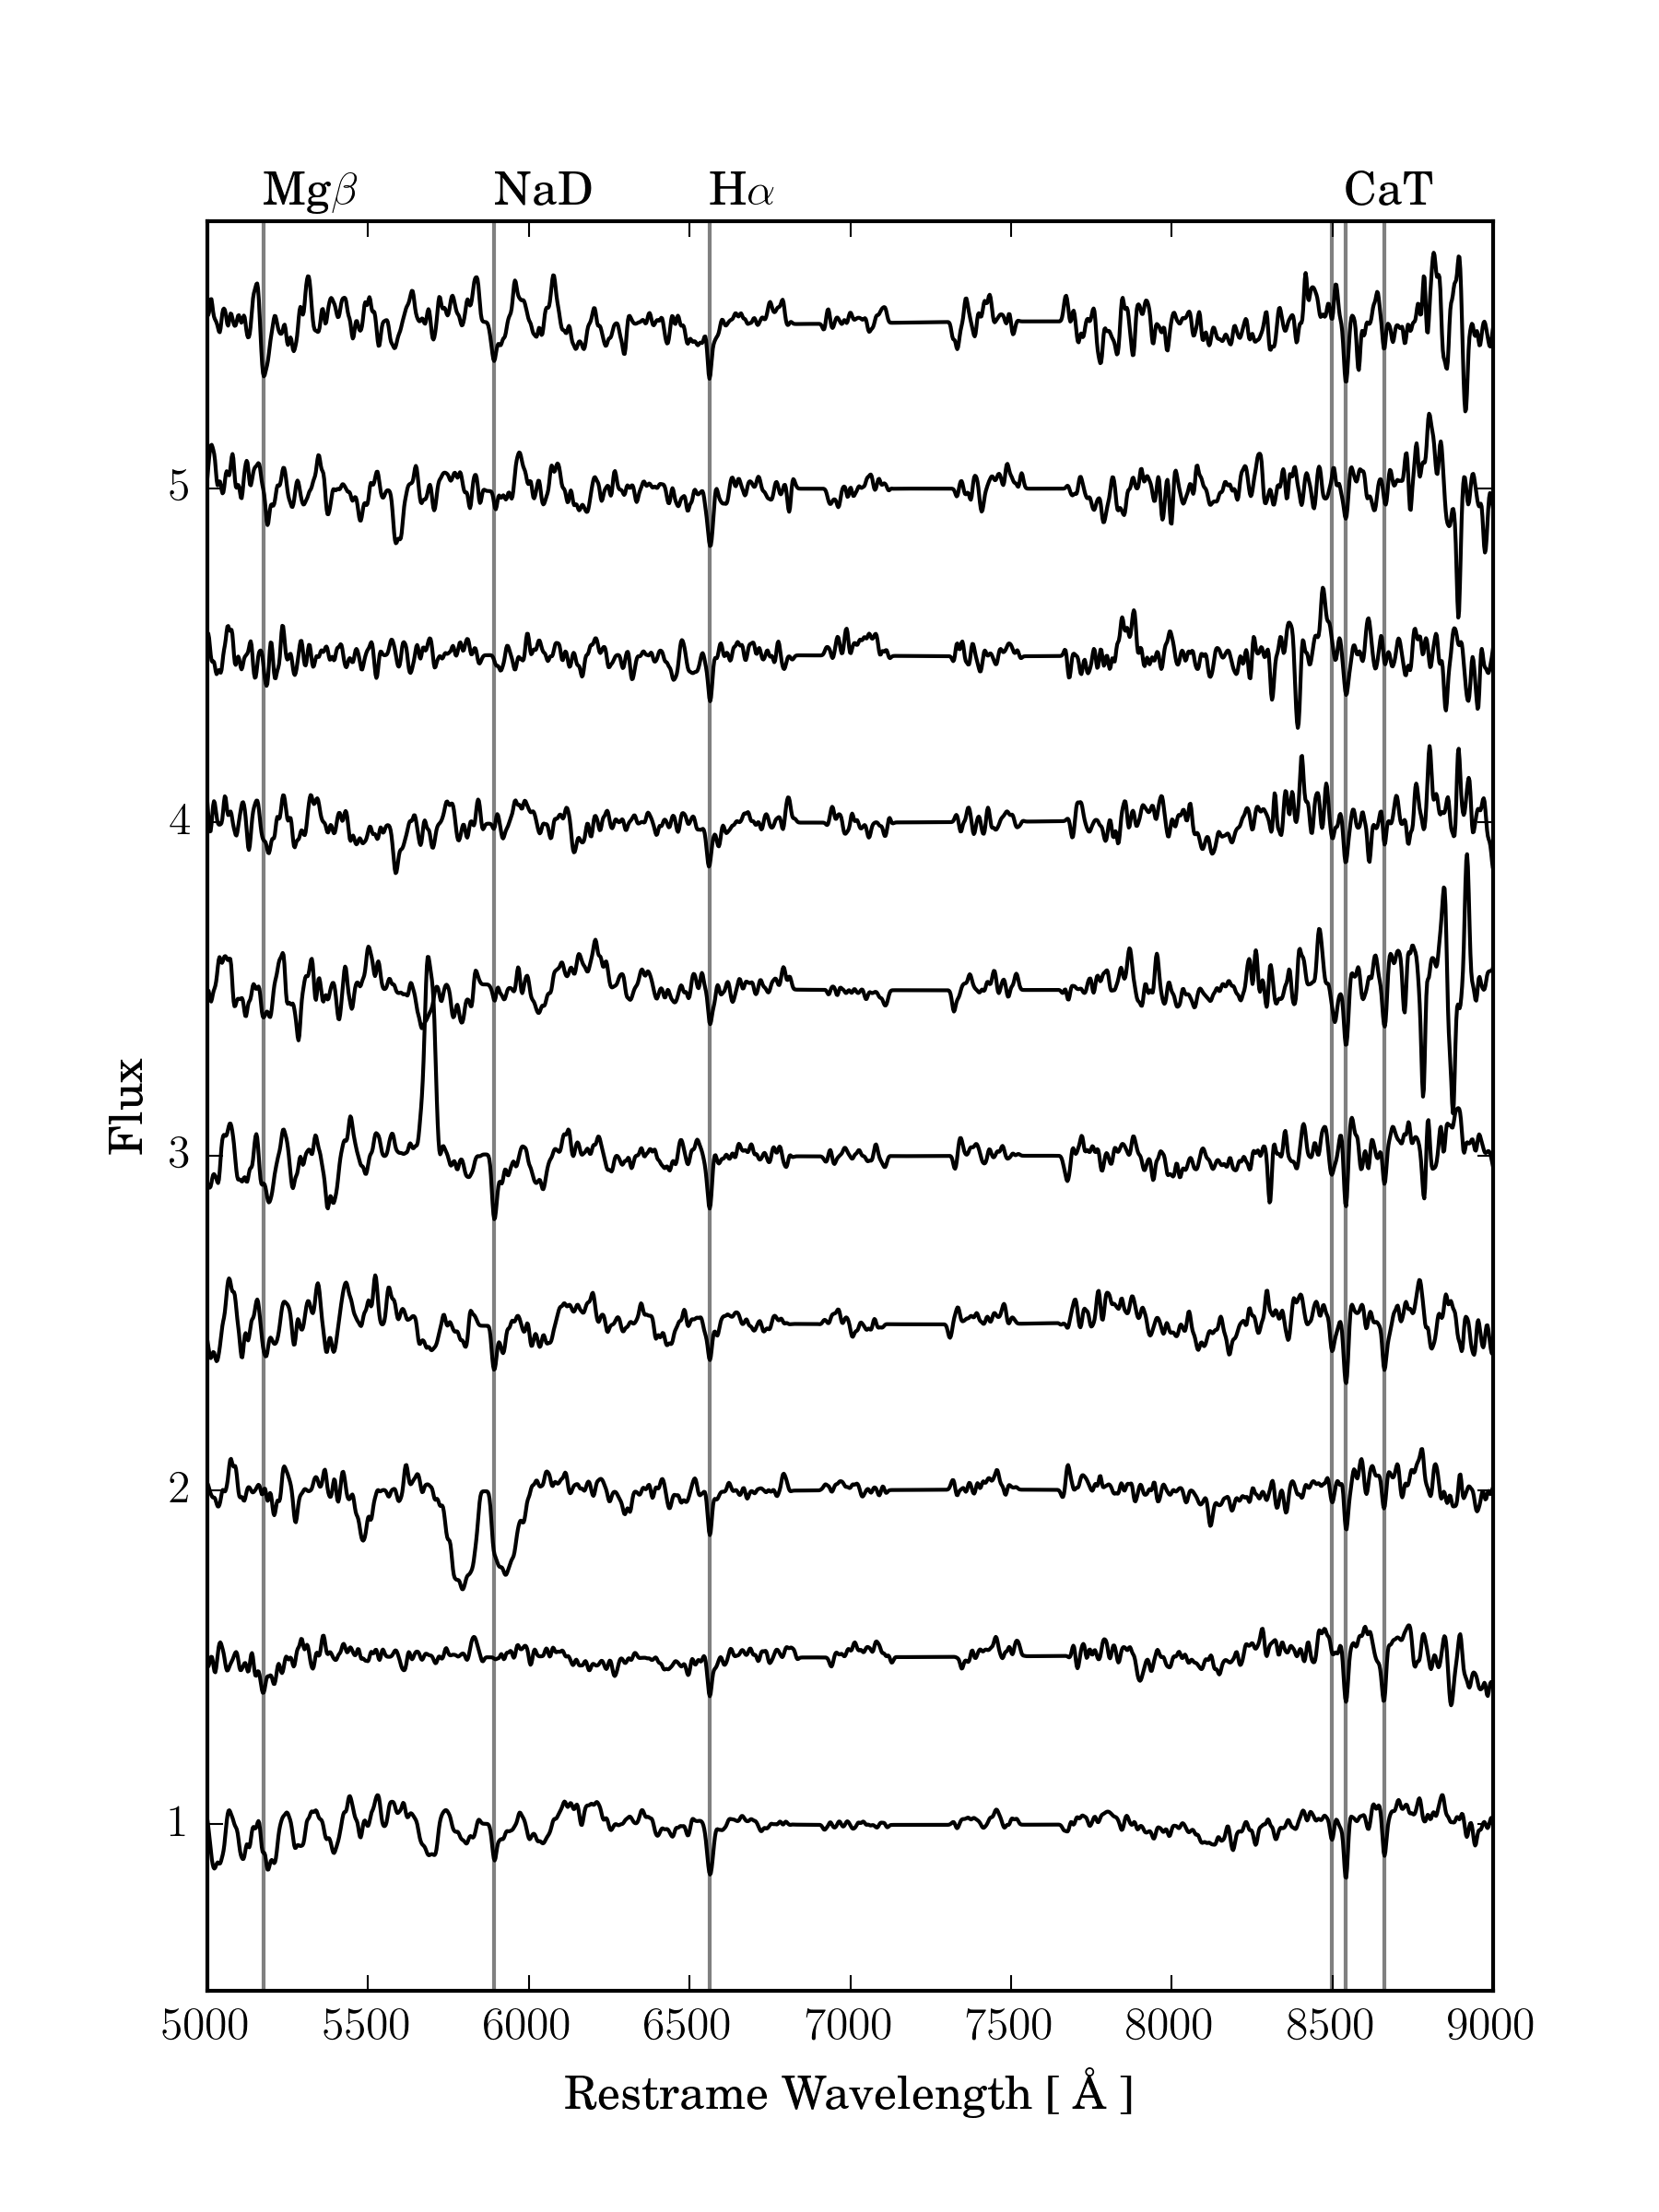
\includegraphics[width=\columnwidth]{figures/vstack_spectra.png} 
\caption{A sample of GC spectra suitably normalised. Shown are continuum-normalized redshift-corrected spectra for GCs with increasing $S/N$ (from top to the bottom). The spectrum at the top has $S/N = 15$, the one at the bottom $S/N = 50$. The main atomic lines are labelled on the top. Features such as the strong absorption in the spectrum at Flux $= 2$ and the emission in the spectrum at Flux $=3$ are instrumental artifacts and not physical features of the GC. The flat horizontal lines between 7000-8000 \AA\ mark regions with masked skylines (see text)}
%NRN: AAron asks "S/N per what? (Ang? resolution element?)"
\label{fig:spectra}
\end{figure}

We used the \citet{Tonry79} R factor (TDR hereafter) to assess the goodness of the correlation between scientific spectra and template spectra. As expected, TDR is inversely proportional to the velocity uncertainties. This effect is shown in Figure \ref{fig:tdr}, where TDR is shown as a function of the measured radial velocity $v$ and velocity uncertainty $\delta v$. 
It is worth noting that {\it fxcor} was set to measure the Doppler shift of the CaT lines only for objects with radial velocities $-500 < v < 3000 \kms$. This means that only radial velocities measured to be $-450 < v < 2500 \kms$ are meaningful, whereas velocities outside this range are non-physical, and thus discarded as meaningless. Heliocentric correction was applied to all radial velocities. 

\subsection{Disentangling Fornax objects from foreground and background contamination}

We are interested in separating objects physically bound to the Fornax cluster (GCs, UCDs and galaxies) from objects unrelated to the Fornax cluster (Galactic stars and foreground or background galaxies). A first distinction can be performed on the basis of the systemic velocity. We use the same velocity range adopted by \cite{Schuberth} for GCs and Galactic stars.
Using the top panel of Figure \ref{fig:tdr} as a reference, Fornax objects are those with $450 \le v <2500 \kms$ (850 datapoints), whereas Galactic stars are those with $-450<v<450 \kms$ (956 datapoints). The velocity determination of background galaxies and their distribution will be discussed in a separate paper.

Spectra of Fornax objects (GCs, UCDs) and Galactic star candidates were redshift-corrected and eyeballed. We checked for the correct positions of the following lines: CaT, H$\alpha (6563 \, \mbox{\AA})$, NaD$(5892 \, \mbox{\AA})$, Mg$\beta (\sim 5175 \, \mbox{\AA})$ and H$\beta (\sim 4861\, \mbox{\AA})$. The CaT and H$\alpha$ lines, if present, are always visible, whereas the Mg$\beta$ line is hardly recognizable in spectra with $S/N \lesssim 10$. The NaD is not always visible because this atomic line is shifted onto a problematic skyline at 5860--5890 \AA\ for spectra with $v \lesssim 1000\kms$ . The H$\beta$ line, at which the instrumental efficiency is less than $20$ per cent, can be discerned only for spectra with $S/N \gtrsim 20 $.

Figure \ref{fig:spectra} showcases some spectra with $S/N$ ranging from 50 (bottom spectrum) to 15 (top spectrum). 
The GG475-filters of the first and third quadrant, coupled with the MR-grism, introduce an absorption feature between about $5600 < \lambda < 6300 \AA\ $ (see the third spectrum from the bottom in Figure \ref{fig:spectra} for an example). This occurs because the GG475-filter is composed of 10-20\% in its weight by sodium oxide. Impure manufacturing likely caused this feature but it does not affect our analysis because the blue part of the spectra is not used for our velocity measurements. Strong emission features can occasionally appear in the blue part of the spectra (see the fifth spectrum from the bottom in Figure \ref{fig:spectra}), but they are attributed to zero order overlaps that are not corrected for by the Reflex reduction pipeline,rather than to physical phenomena associated with the light source. 

For spectra with very low $S/N$ the distinction between atomic lines and noise features becomes somewhat subjective. Therefore, all 850 Fornax object candidates were independently eyeballed by five members of the team. The inspection was performed on a dashboard including the 2D image of the source, the redshift corrected spectrum and attributes such as magnitude and S/N. We gave a vote of $1$ to spectra which were certainly Fornax objects and $0$ to non-Fornax object spectra. We found that 323 spectra received a vote of 5/5 (meaning that these spectra were classified as Fornax objects by all members of the team), 348 spectra received a vote of 4/5 and 420 spectra received a vote of 3/5. In the followings, we will use the last set of 420 spectra as our final spectroscopic catalogue of the Fornax cluster. 

We repeated the above procedure to select a sample of spectroscopically confirmed Galactic stars with radial velocities in the range $-450<v<+450 \kms$, finding a total of 492 Galactic stars.

\section{Results}
\label{sec:analysis}
\subsection{Velocity self-consistency}

We measured radial velocities for 51 duplicated objects (including Galactic stars), observed across multiple VIMOS masks. The velocity difference $\Delta v$ between duplicated objects is shown in Figure \ref{fig:internal} as a function of $g$ magnitude. We detected no clear trend between $\Delta v$ and the magnitude. One object has a velocity difference which scatters more than 3$\sigma$ from the average. We attributed this disagreement to an issue with the wavelength calibration for this particular object. The root-mean-square of the velocity difference (of GCs and stars combined) is $91 \kms$, which becomes $79\kms$ after clipping the outlier. 

We averaged the radial velocities of the duplicated GCs and summed in quadrature their velocity uncertainties. This left us with a catalogue of 387 Fornax objects and 464 Galactic stars.

\begin{figure}
\centering
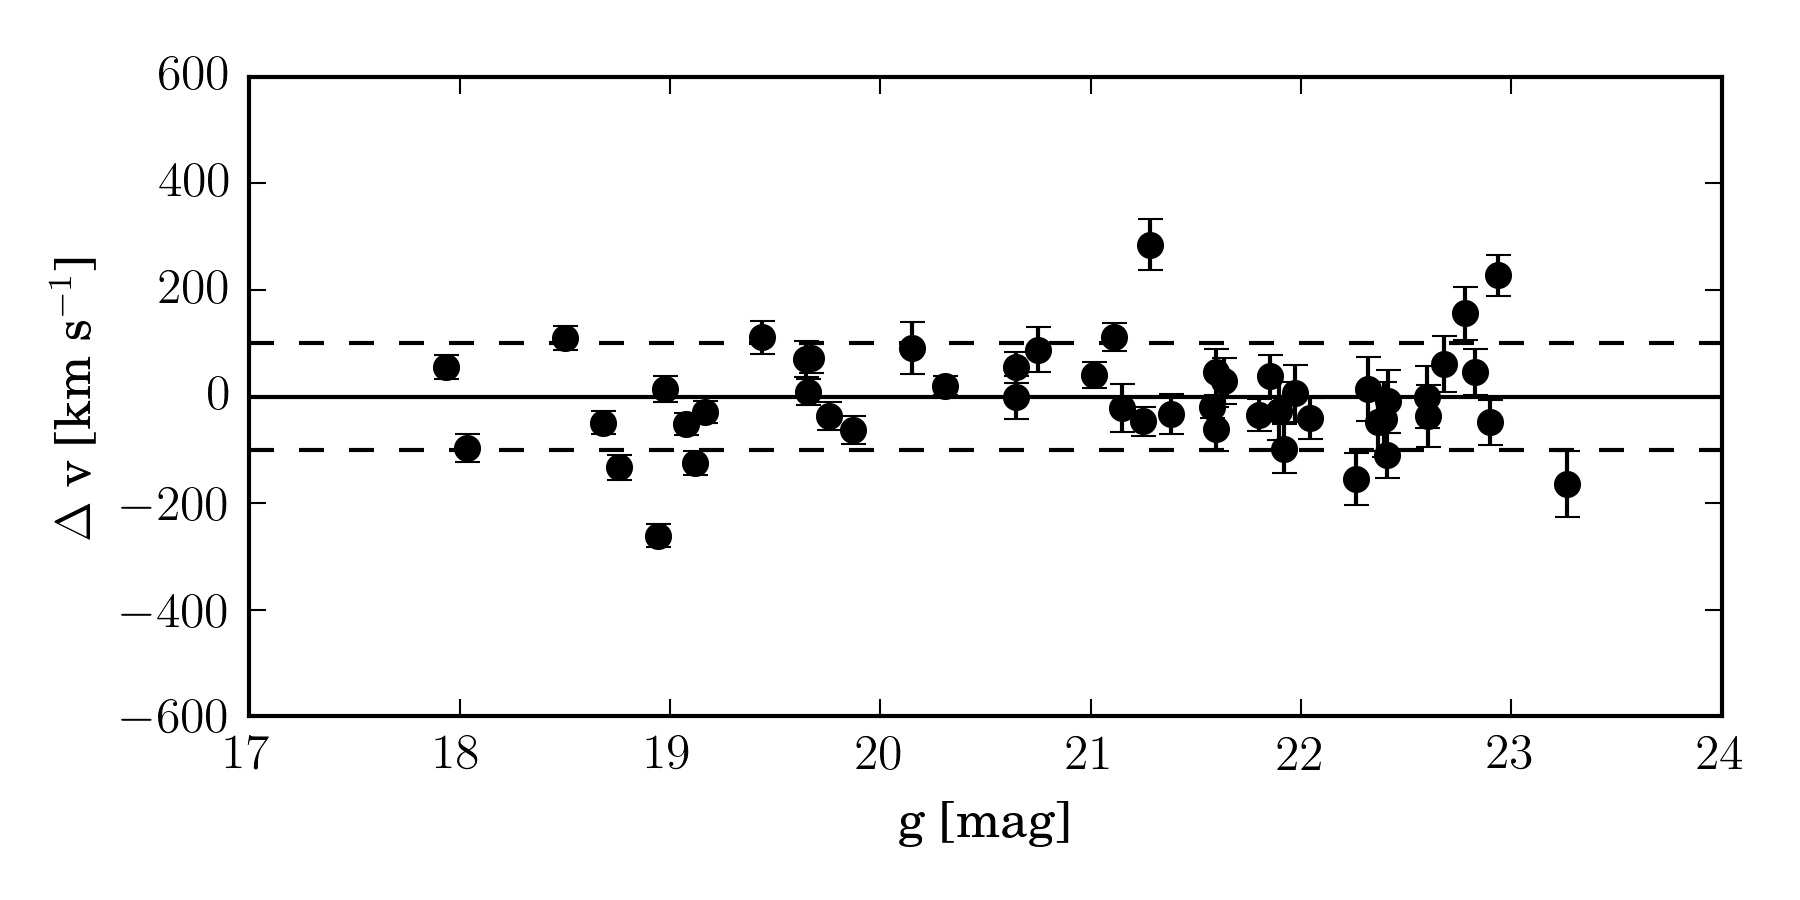
\includegraphics[width=\columnwidth]{figures/internal.png} 
\caption{Internal velocity comparison. The figure shows the velocity difference $\delta v$ between GCs with two independent velocity measurements. The solid and dashed line represent $\delta v = 0 \kms$ and $\delta v = \pm 100 \kms$, respectively. }
\label{fig:internal}
\end{figure}

\subsection{Comparison with literature data}

The stellar systems surrounding NGC~1399 has been in the focus of many spectroscopic studies
\citep{Dirsch04, Schuberth10, Bergond07, Firth07, Chilingarian11, Mieske04, Hilker07, Francis12, Drinkwater00}.

To find which of our VIMOS objects have a literature counterpart, we matched our catalogue of 387 Fornax objects with the NED (Nasa/Ipac Extragalactic Database\footnote{https://ned.ipac.caltech.edu/ .}) database using the python/astropy tools. 
We manually added the catalogue of \citet{Schuberth} to the literature database, because these GC measurements are not in NED. We required the literature objects to have a measured radial velocity and to be within 0.4 arcsec from our VIMOS source. 

In most cases, the literature counterpart has been observed by more than one author. Table \ref{tab:authors} reports the number of objects per author for which we have a VIMOS radial velocity. 
In order to compare literature velocities with our VIMOS velocities, we averaged together the radial velocities of unique objects observed in multiple literature studies. Uncertainties were summed in quadrature. 
%NRN: do you mean subracted off in quadrature??? see also in Sec 5.3
Overall, we found 48 of our Fornax objects to have a literature counterpart. 

Figure \ref{fig:vel_comparison} shows the comparison between the our VIMOS objects and the unique literature objects obtained as explained above. Also in this case the agreement is satisfactory and no systematic bias is detected. 

%There exist two archival GC catalogues of NGC~1399. The one from \citep{Schuberth} contains 693 unique GCs, obtained using medium resolution spectroscopy from VLT/FORS2 and Gemini-South/GMOS. This catalogue includes sources within 18 arcmin from NGC~1399 and a magnitude range of $19.5<r<23.5$ mag. The second catalogue is the one from \citet{Bergond07}, which used VLT/FLAMES in low resolution mode to confirm 149 GCs. Bergond's catalogue was designed to target intra-cluster globular clusters and it is therefore more radially extended. It covers a strip of about one degree in right ascension and half a degree in declination. 

%We matched the position of our GCs (and Galactic stars for the Schuberth's catalogue) with the position of literature objects to test how radial velocities compare with each other. Results are shown in Figure \ref{fig:vel_comparison}. Overall, the agreement with the literature is satisfactory. We found 48 GCs and 31 Galactic stars in common with the Schuberth catalogue. The root-mean-square of the velocity difference is $81\kms$ and $96\kms$ for GCs and Galactic stars, respectively. We found 16 GCs in common with the Bergond catalogue, with a root-mean-square of $46 \kms$. 

\begin{figure}
\centering
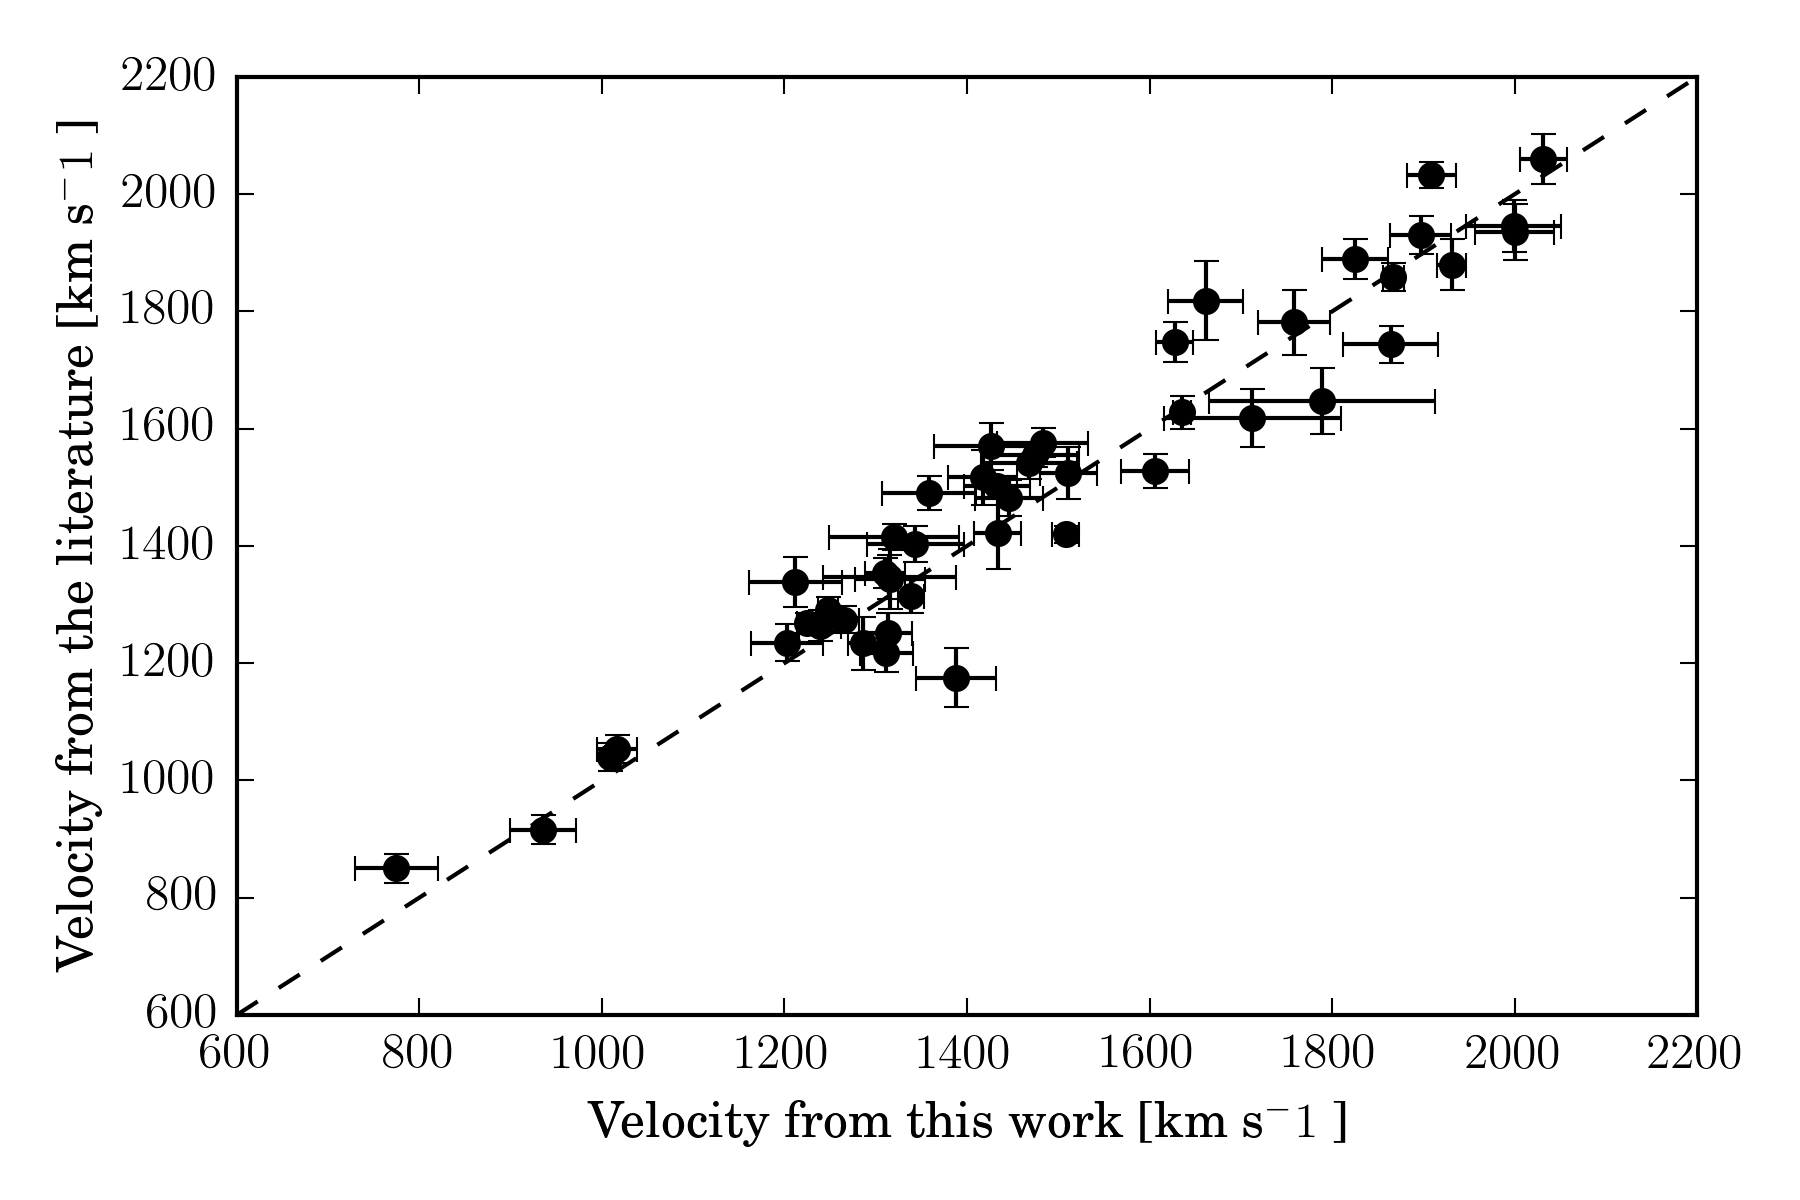
\includegraphics[width=\columnwidth]{figures/vel_literature.png} 
\caption{Comparison with literature studies. The radial velocity of literature objects is averaged among literature studies as discussed in the text. The 1 to 1 line is shown as a dashed line. }
\label{fig:vel_comparison}
\end{figure}
%NRN: Aaron coments about fig. 5 and 6: agreement is not satisfactory within the error bars in these plots ! I guess the plots show no biases but a significant scatter (which we comment to be ~80 km/s). I guess this represents our statistical error (has this been subtracted of the Vrms in Fig. 9????) 
\begin{table}
\centering
\label{mathmode}
\begin{tabular}{@{}l c}
\hline
Paper & Number of duplicated objects \\
\hline
\citet{Dirsch04} &         29 \\
\citet{Schuberth10} &       26 \\
\citet{Bergond07}  &     14 \\
\citet{Firth07}   &      11 \\
\citet{Chilingarian11} &     2 \\
\citet{Mieske04} &       1 \\
\citet{Hilker07}  &     1 \\
\citet{Francis12}   &     1 \\
\citet{Drinkwater00}  &    1 \\
\hline
\end{tabular}
\caption{Number of confirmed VIMOS objects also found in archival data (grouped by author). }
\label{tab:authors} 
\end{table}

\subsection{Classification of Fornax objects}

We classified all Fornax objects based on their morphology: namely GCs, ultra compact dwarfs (UCDs) and background galaxies. The spatial resolution of VST/OmegaCam is insufficient to resolve the typical half-light radii of GCs with $r_h < 10$ pc \citep{Masters, Puzia11}. Although the size of UCDs with $r_h > 20$ pc can be resolved using our imaging data \citep{Cantiello15}, measuring UCD sizes is not the focus of this paper and will be deferred to a future work.

It is established that a sharp magnitude cut cannot perfectly separate UCDs from GCs ({\bf MN: reference?}). However, it has been shown \citep{Voggel16, Eigenthaler18} that the bulk of UCDs with confirmed sizes in the Fornax cluster have $M_V \le 10$ ($\approx M_i \le 11$). 
%NRN: Aaron comment: where is this in their paper?  I have a feeling it's not right, and includes a lot of GCs as well as UCDs; I would suggest calling these "candidate UCDs"
Therefore, we use this magnitude cut as benchmark value to separate UCDs with $i \le 20.3$ from GCs with $i > 20.3$. This selection returns 15 UCD candidates and 372 likely GCs. 

The object at $\alpha=$3:36:37.253 $\delta=-$35:23:09.20 is the nucleus of the nucleated dwarf galaxy FCC~171, whose radial velocity was first measured in \citet{Bergond07}. This object will be treated as a GC in the following analysis.  
%NRN: Aaron comment why?? it's not a GC!
%Our catalogue also includes the UCD FCSS J033854.1-353333,  with radial velocity $v_r = 1492 \kms$ \citet{Chilingarian11}. 

\section{Discussion}
\label{sec:discussion}
In this section we discuss some qualitative properties of the final dataset. We look at the spatial distribution and phase-space diagrams. A detailed kinematic and dynamic analysis (rotation curve, dark matter modelling, luminosity function analysis) will be the subject of forthcoming papers.

\begin{figure*}
\centering
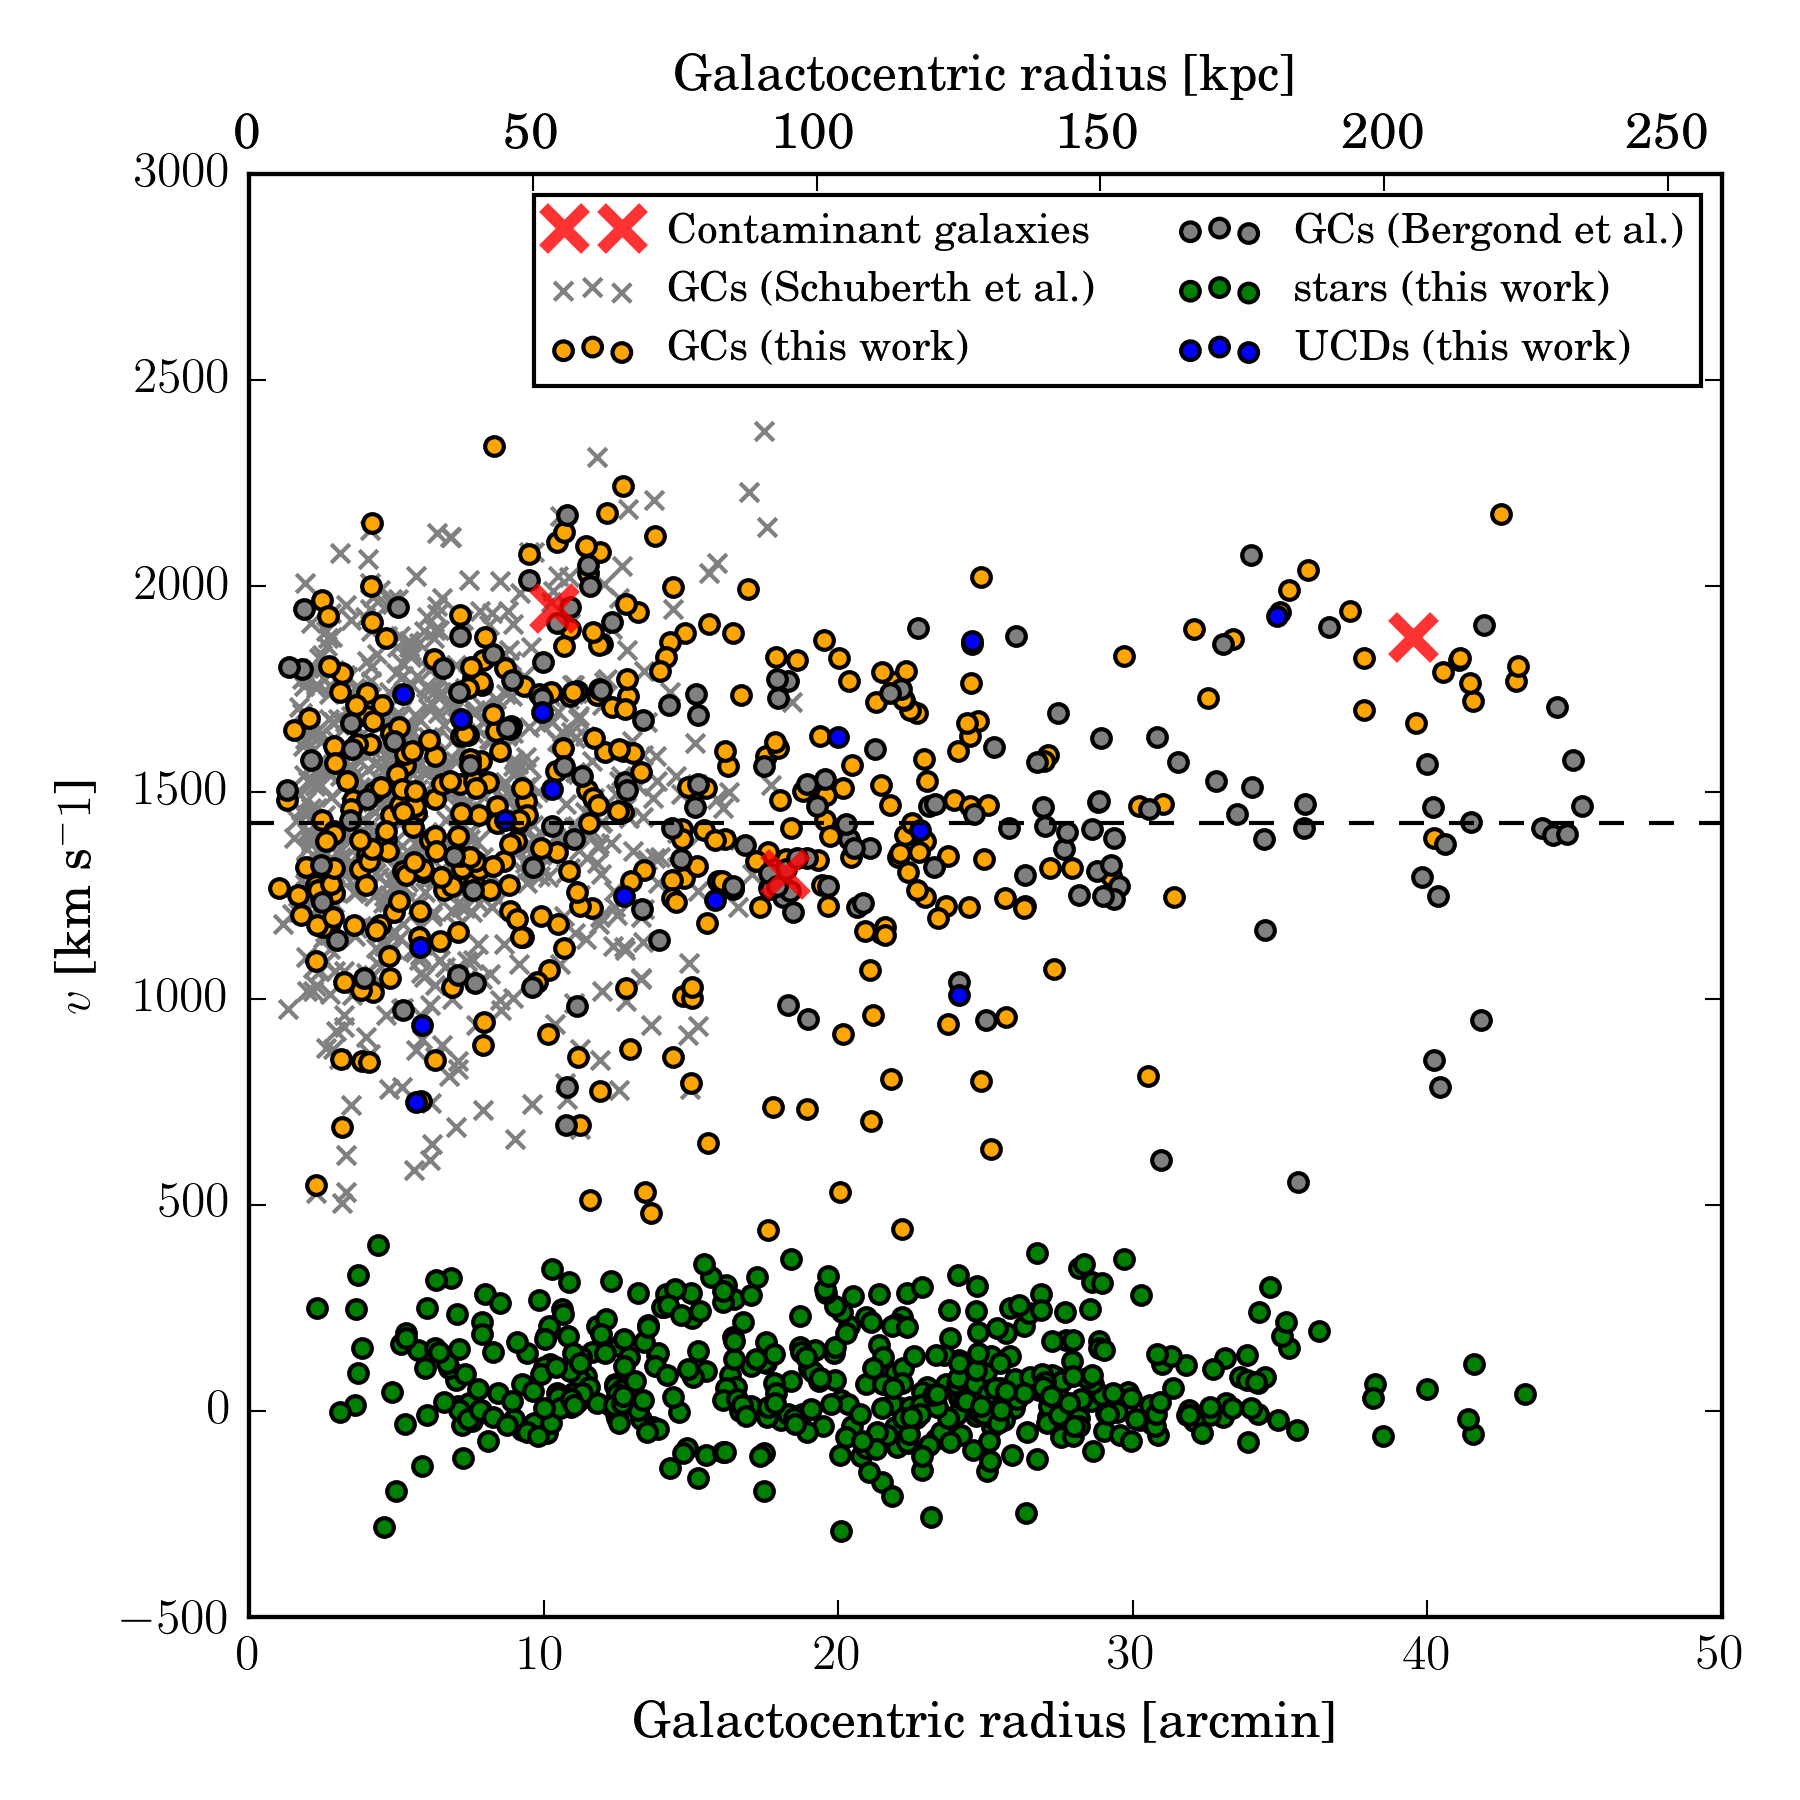
\includegraphics[width=\columnwidth]{figures/RV.png} 
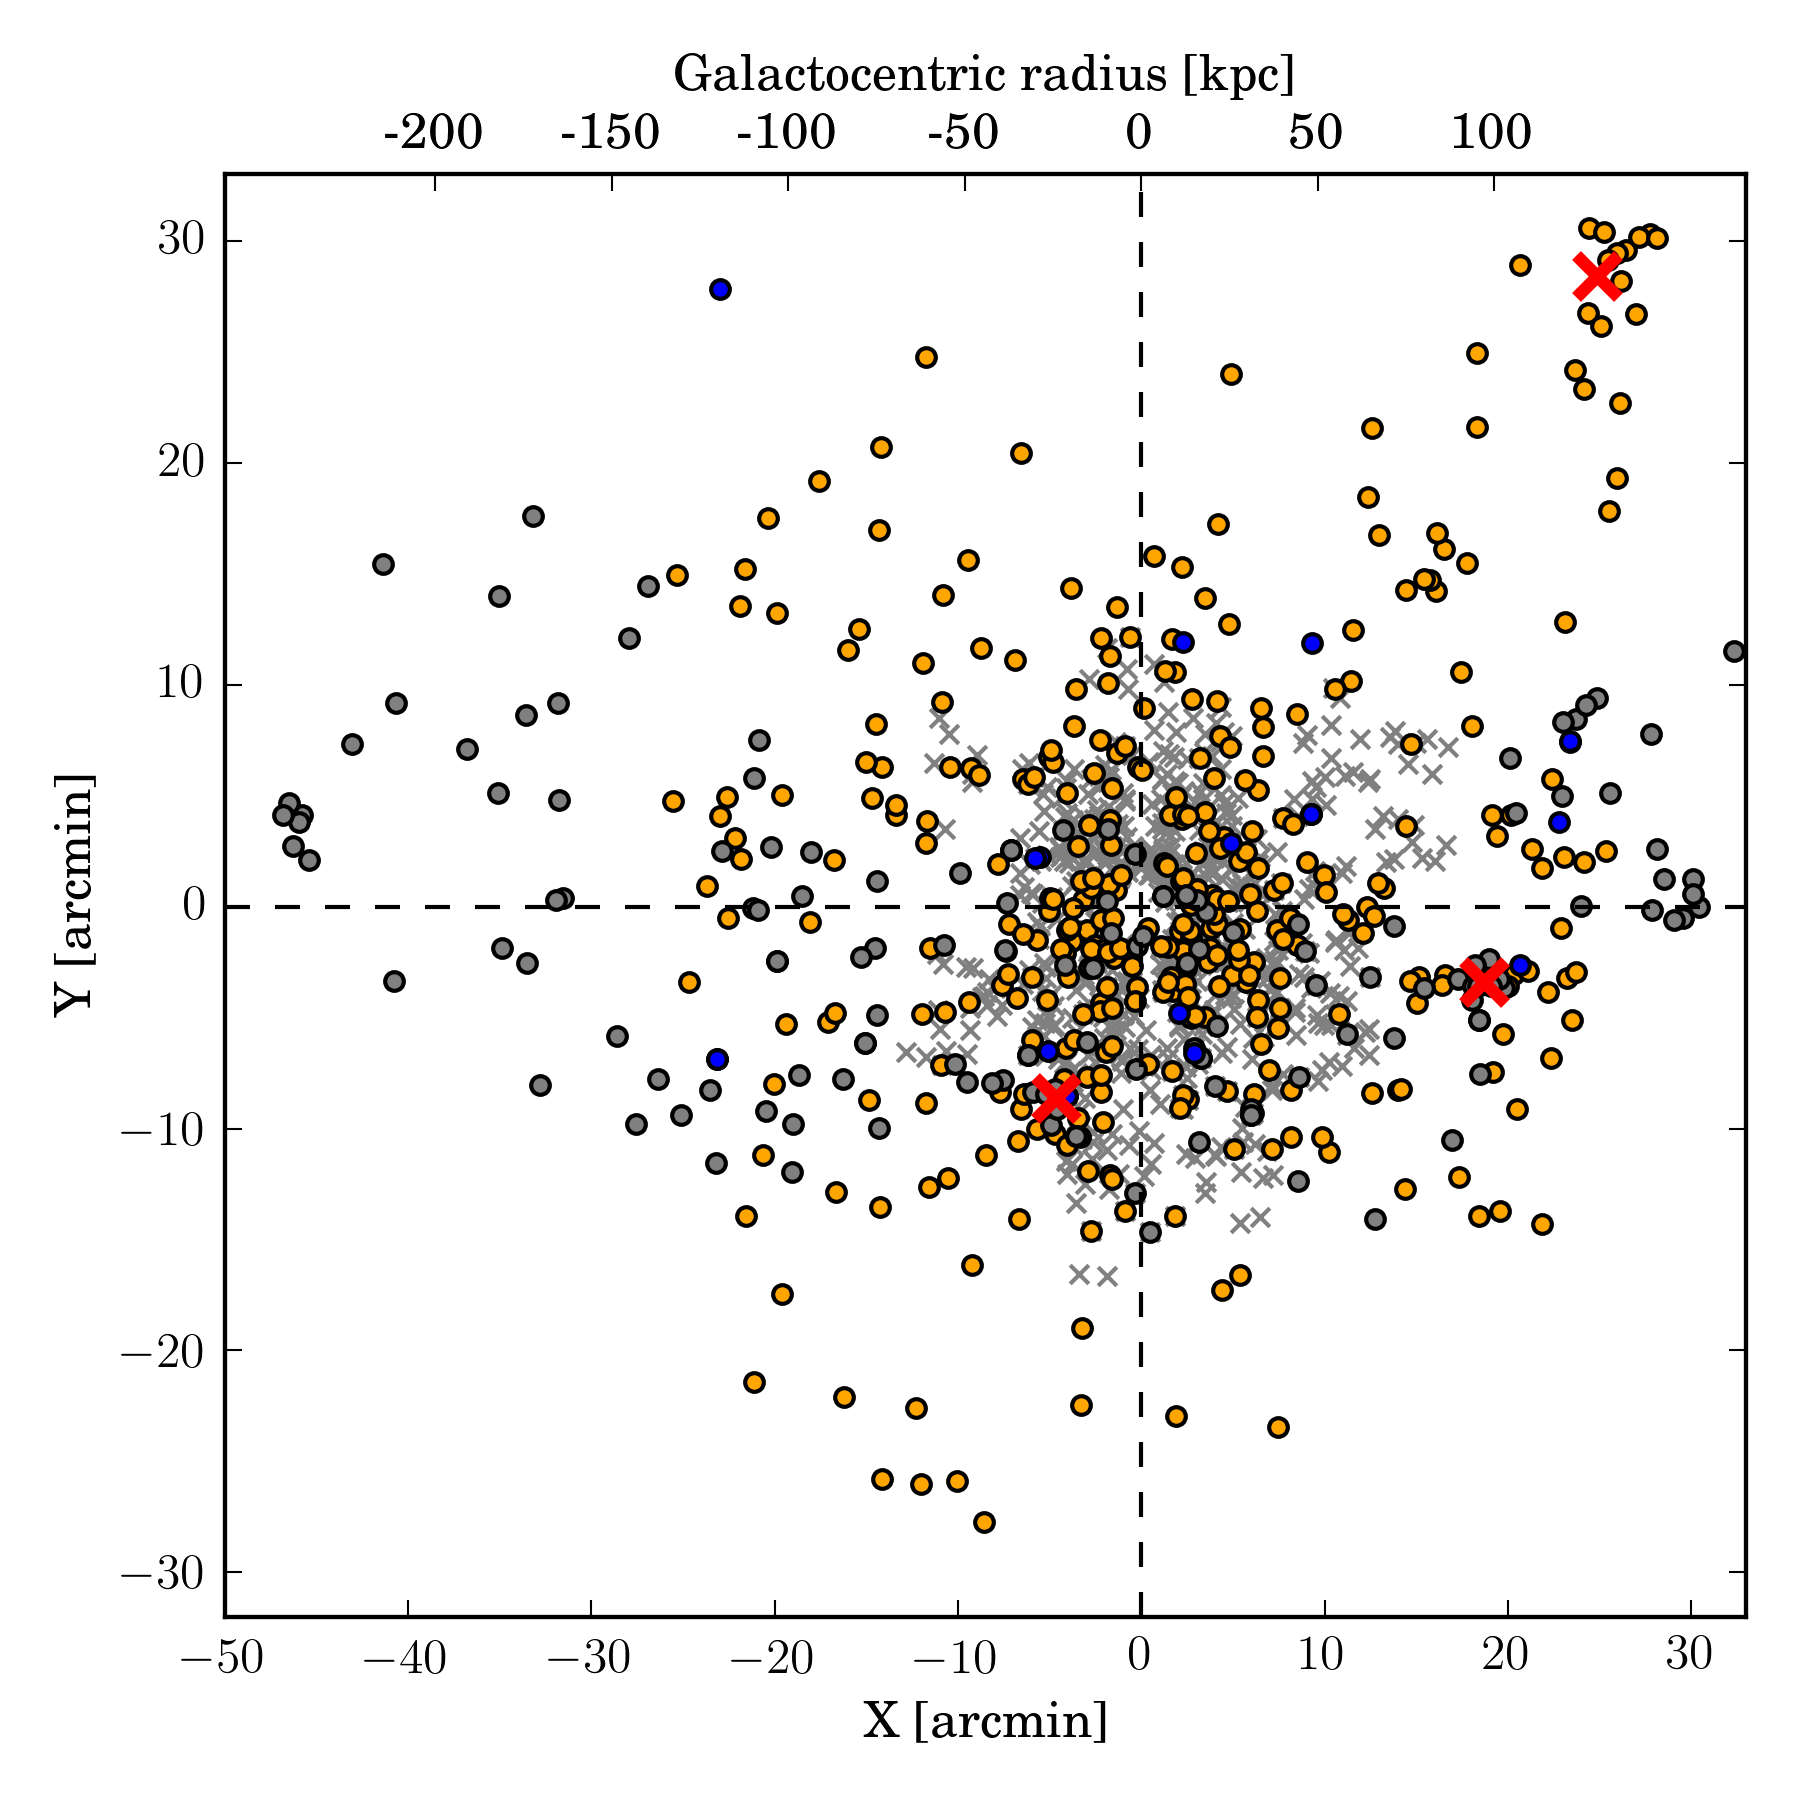
\includegraphics[width=\columnwidth]{figures/XY.png} 
\caption{\textit{Left}: Phase-space velocity diagram. The figure shows the measured systemic velocity of the Fornax objects presented in this paper (orange points), GCs from \citet{Schuberth} (grey crosses), GCs from \citet{Bergond07} (greys points) and Galactic stars measured in this paper (green points). The systemic velocity of NGC~1399 is marked with a dashed line at $v = 1425$ km s$^{-1}$. The systemic velocity and galactocentric distance of giant Fornax galaxies (namely NGC~1404, NGC~1387, NGC~1380) are shown as red crosses. Physical distances in kpc are also shown on the top panel. \textit{Right}: Position diagram, with North to the top and East to the left. The plot shows the spatial distribution of the objects from the left panel (except for Galactic stars for clarity). The distance is expressed in arcminutes from the centre of NGC~1399. Physical distances in kpc are also shown on the top panel.  Note how the GCs from our paper complement the GC catalogues of \citet{Schuberth} and \citet{Bergond07}. }
%CS: Would it be easy to put the names of the galaxies on top of the red crosses? So that the reader knows who is who!
\label{fig:phase-space}
\end{figure*}

\subsection{Phase-space and spatial distribution}

The phase-space diagram and the spatial distribution are shown in Figure \ref{fig:phase-space}. In both cases, GCs, UCDs and Galactic stars are compared to the catalogues of \citet{Bergond07} and \citet{Schuberth}. These two catalogues are the largest and most homogeneous in the literature. Moreover, the catalogue of Schuberth is an extension of the catalogue of \citet{Dirsch04}. Together they include sources within 18 arcmin from NGC~1399. Bergond's catalogue was designed to target intra-cluster globular clusters and it is more radially extended (see also Figure \ref{fig:fov}). It covers a strip of about 1.5 degree in right ascension and half a degree in declination. The catalogues of Schuberth and Bergond combined provide a good representation of the current archival phase-space and spatial distribution of the GC system in the core of the Fornax cluster. 

The left panel in Fig. \ref{fig:phase-space} shows that the velocity distribution of GCs/UCDs is well separated from that of Galactic stars, although a few GCs between $10<R<20$ arcmin might be misclassified as Galactic stars. 

The systemic velocity of GCs and UCDs is $v_{\rm GCs} = 1443 \pm 18 \kms$ and $v_{\rm UCDs} = 1413 \pm 91 \kms$, respectively. These are both consistent with the average systemic velocity from the literature $v_{\rm NED} = 1425 \pm 4 \kms$. Our sample also includes interlopers from large galaxies surrounding NGC~1399, in particular NGC~1380, NGC~1404, NGC~1387. The positions of these three galaxies in the phase-space diagram are marked with red crosses. 

It is not trivial to disentangle the GC population of NGC~1387 and NGC~1404 because of their proximity in phase-space to NGC~1399. 
Here we adopt a conservative approach to extract the GC system of these galaxies, but we acknowledge that more complex methodologies can return more accurate results. Following \citet{Schuberth}, we use 3 arcmin from the galaxy centre as a benchmark radius to select the bulk of GCs associated with these galaxies. We also require that the radial velocity of the GCs should be within $v_{\rm sys} \pm 2\sigma$  the systemic velocity of the host galaxy, where $\sigma$ is the galaxy stellar velocity dispersion. Here we used $\sigma = 247 \kms$  \citep{Vanderbeke11}, $v_{\rm sys} = 1947 \kms$ for NGC~1404 and $\sigma = 170 \kms$ \citep{Wegner03}, $v_{\rm sys} = 1302\kms $ for NGC~1387, respectively. After applying the above selection criteria, we found 17 and 8 GCs associated with NGC~1404 and NGC~1387, respectively. The larger number of GCs associated with NGC~1404 is due to the galaxy being more massive than NGC~1387, but also to its proximity to NGC~1399 which increases the fraction of contaminants.
In the case of NGC~1380, with $\sigma = 190 \kms$  \citep{Vanderbeke11} and $v_{\rm sys} = 1877 \kms$, the identification of its GC system is easier given its isolated position. Using the criteria above, we found 7 GCs associated with this galaxy. 

The right panel of Figure \ref{fig:phase-space} displays the spatial distribution of our GC and UCD catalogues. This diagram also shows how our catalogue is complementary to literature catalogues: it increases the object sampling in the central regions of the galaxy and it fills gaps with no data in the outer regions. 

GC systems which are bound to other giant galaxies can be seen clustered around their centres. Figure \ref{fig:phase-space} suggests that our combined sample might also contain some GCs belonging to NGC~1379 and NGC~1381 (see Figure \ref{fig:fov}). 
%CS: if it is not too complicated, I think it would help to add the names of the galaxies into the plots and for the right panel, it makes sense to also add NGC1379 and NGC1381, without sending the reader back to Fig.1

%NRN: comment form Aaron: those galaxies should be marked in Fig 7 somehow, not just in Fig 1; also, these GCs come from Bergond+07: did they not discuss this issue?

\begin{figure*}
\centering
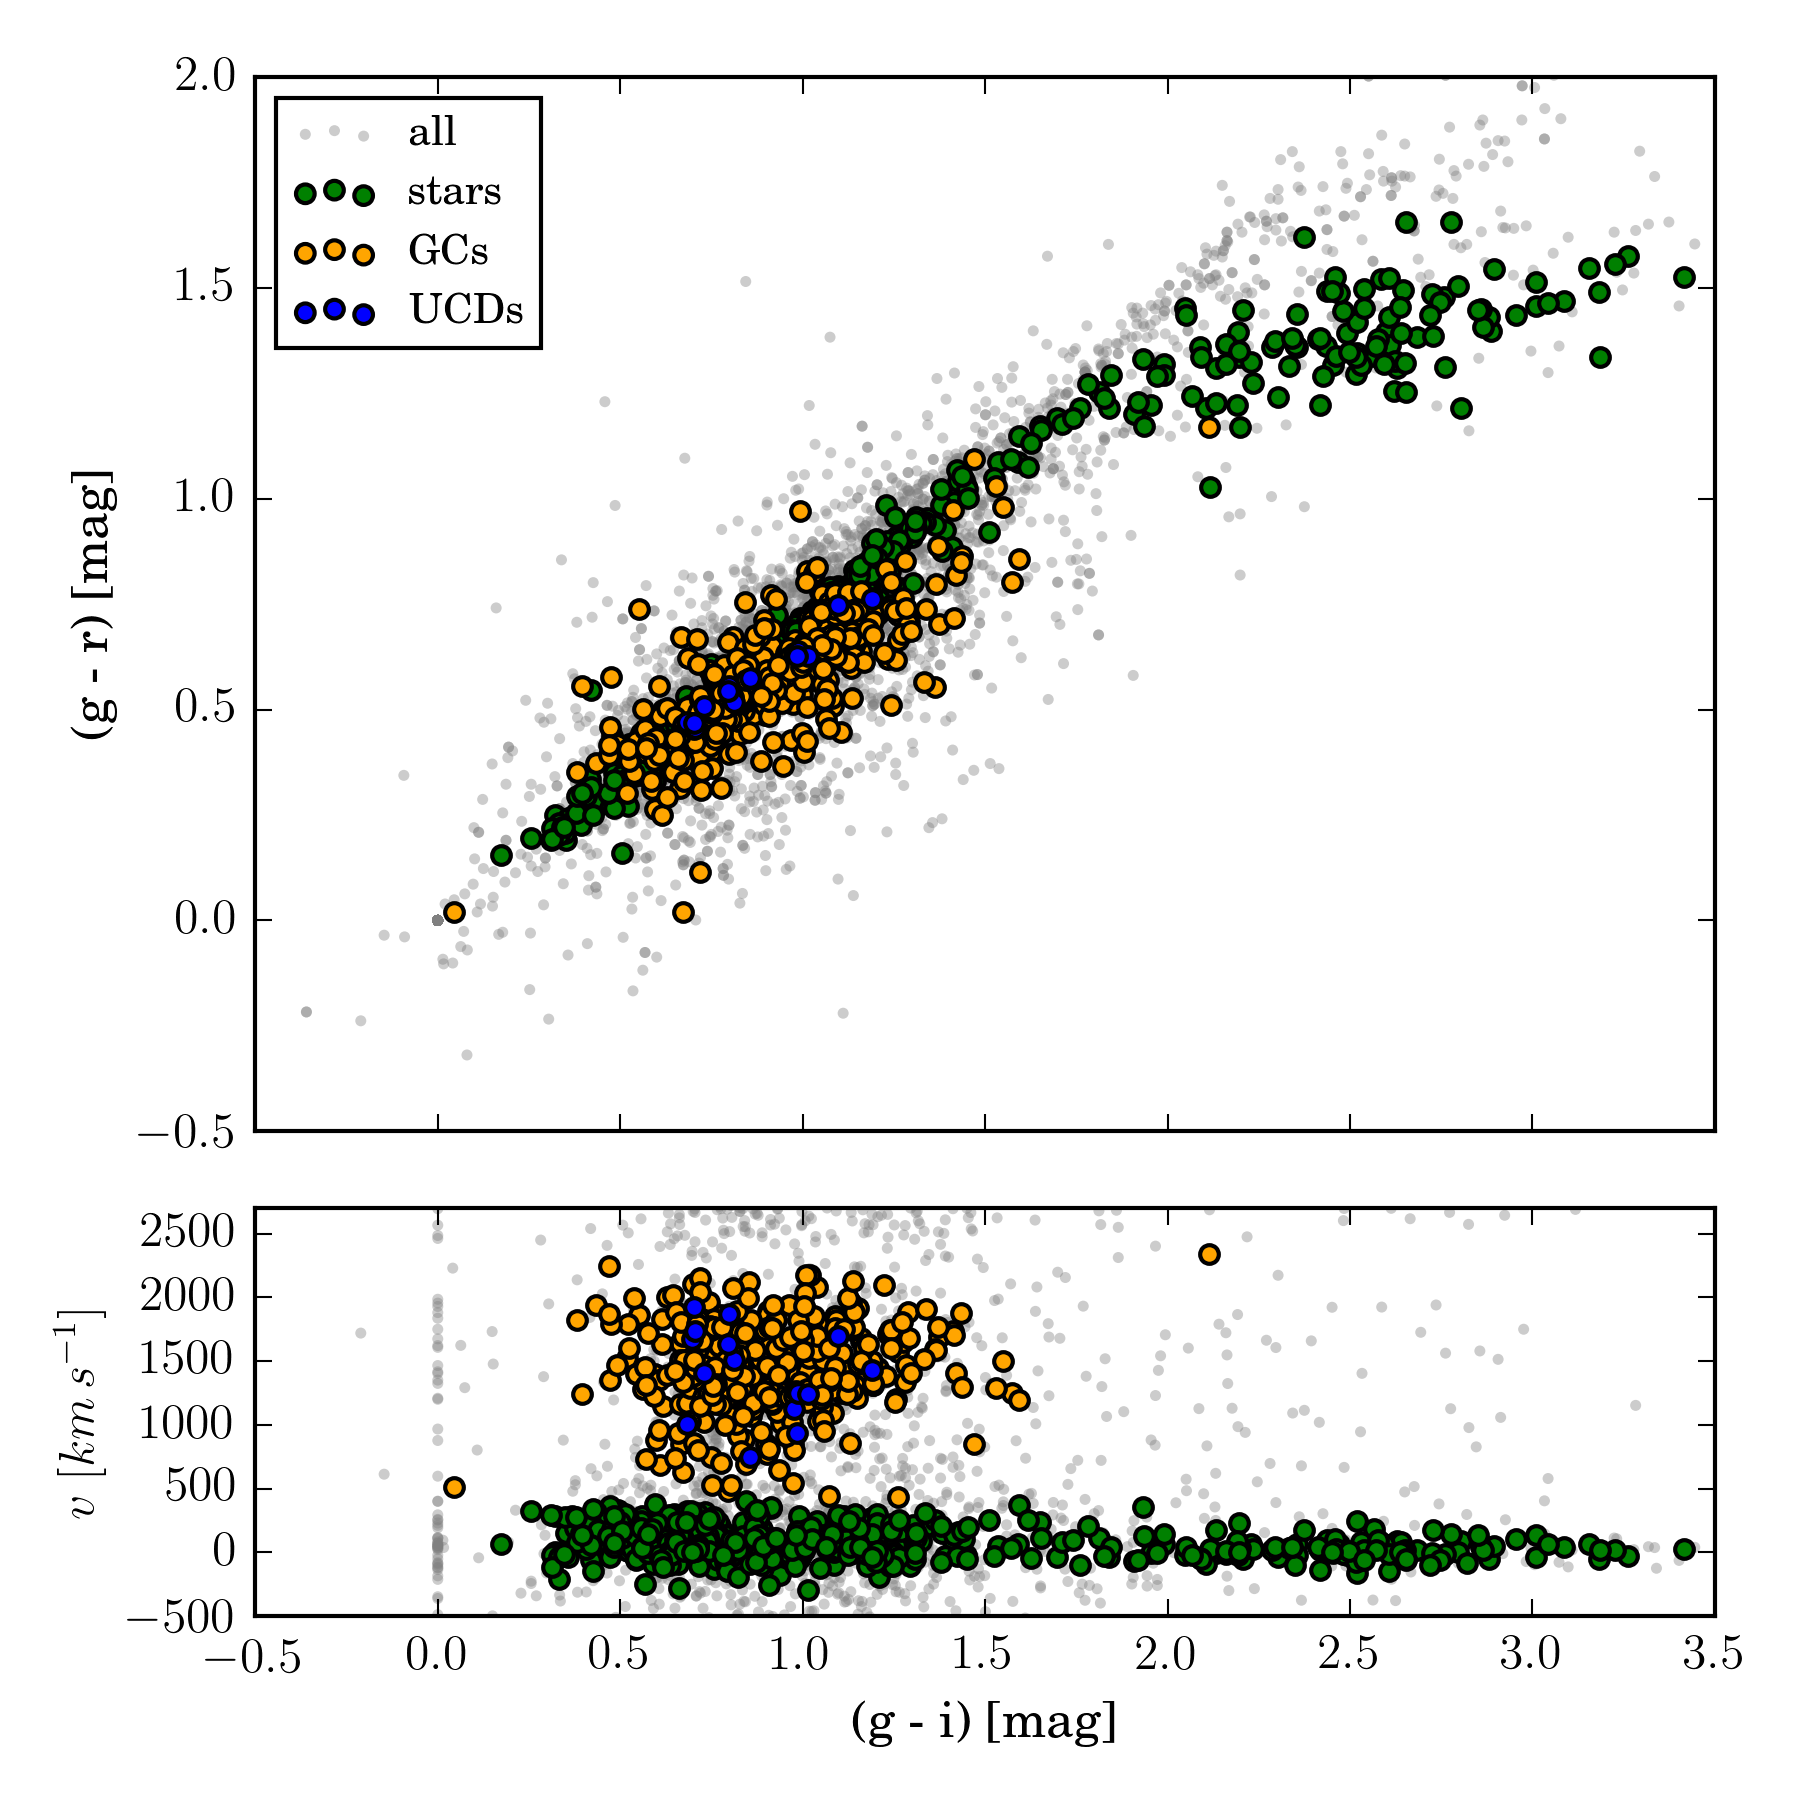
\includegraphics[width=\columnwidth]{figures/cc.png} 
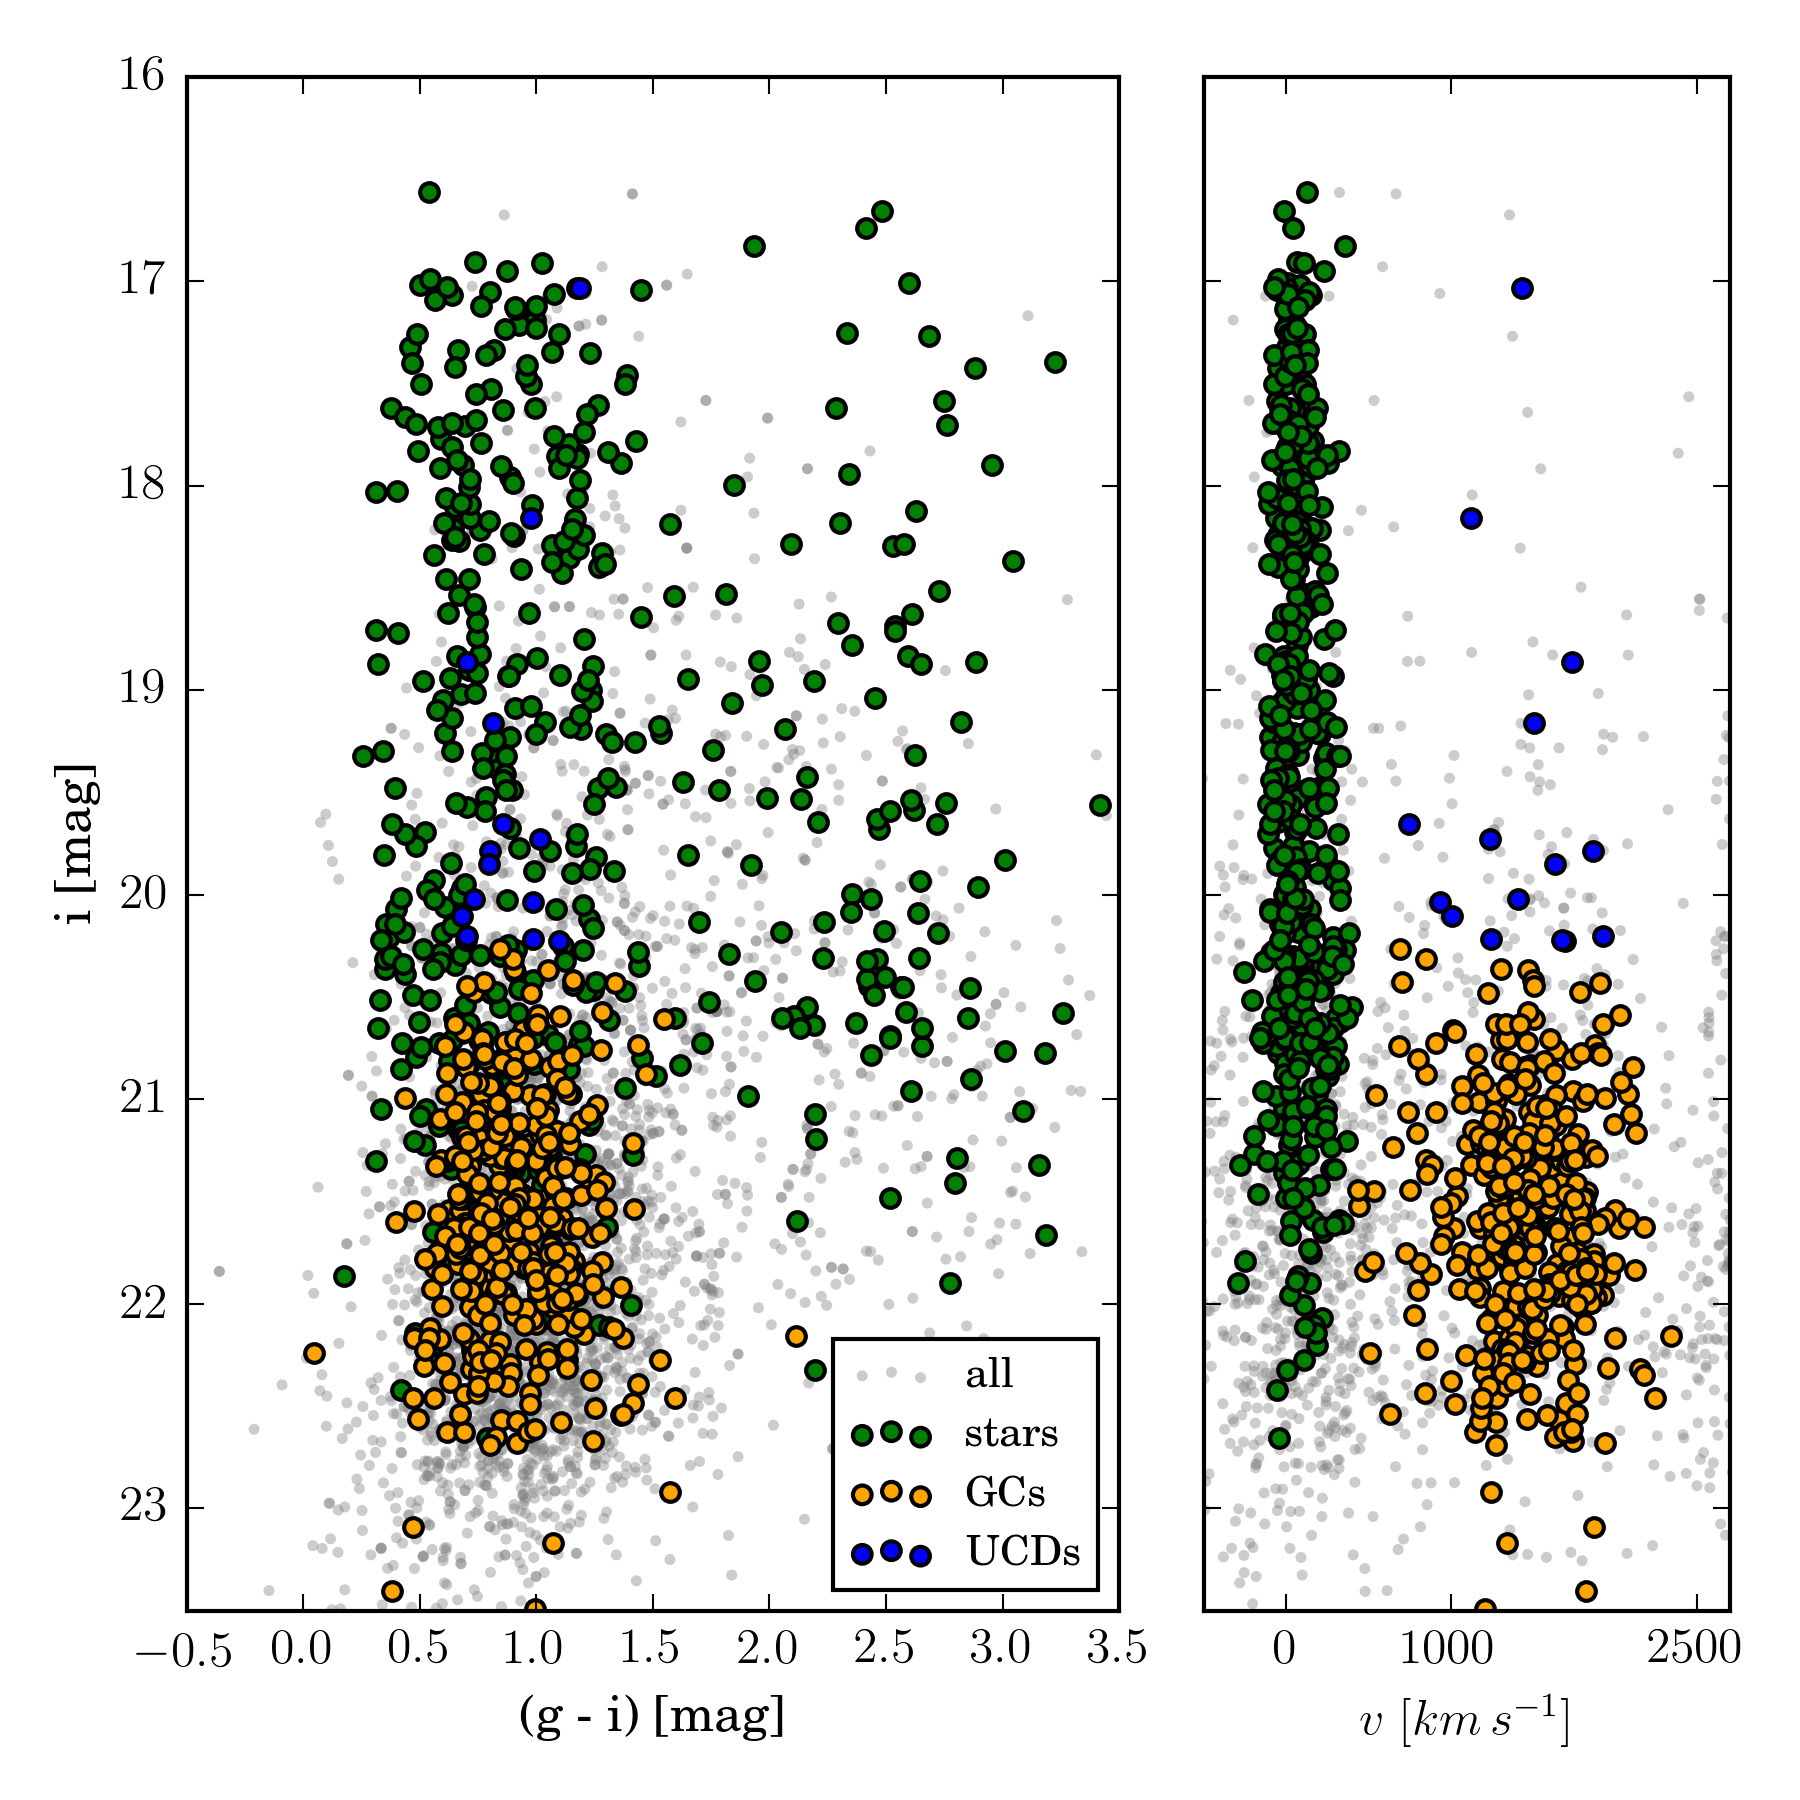
\includegraphics[width=\columnwidth]{figures/cm.png} 
\caption{Colour--colour and colour--magnitude diagram. The figure shows the distribution of the labelled objects in a $(g-i)$ vs. $(g-r)$ space (left panel) and $(g-i)$ vs $i$ space (right panel). Each diagram includes also a radial velocity $v$ axis to show the separation of GCs/UCDs from stars and galaxies. The objects labelled as 'all' represent all sources targeted for spectroscopic follow-up and not the photometric master catalogue. {\bf check the discrepant object pointed by MN}. }
%NRN: comment form Aaron: it seems odd that there were all these grey points on a separate track that were observed but no velocity found(?) -- what are they?
\label{fig:cc}
\end{figure*}

\subsection{Photometric diagrams}

%\citet{DAbrusco16} used the same photometric dataset we used in this paper to show that the colour distribution of GCs in NGC~1399 is bimodal, as found in all giant galaxies. Bimodality usually translates into different physical properties of the blue (metal-poor) and red (metal-rich) GCs, such as spatial distribution, kinematics which are probably linked to different formation scenarios. 

Figure \ref{fig:cc} displays the distribution of GCs/UCDs in the photometric space. These are compared with the distribution of all sources targeted for spectroscopic follow-up, including Galactic stars and background galaxies. Although the $u$ filter is known to well discriminate GCs from contaminants, here we only consider $g$, $r$, $i$ magnitudes because all but one GCs/UCDs have a genuine measurement in these photometric bands, whereas only 50\% of our GCs/UCDs have a $u$-band measurement. This is due to $u$-band imaging being shallower than the other bands for detecting faint GCs \citep{DAbrusco16}.

GCs/UCDs and contaminants are not well separated using merely $g$, $r$, $i$ filters, but velocity information clearly separates GCs/UCDs from Galactic stars and background galaxies. This is also shown in Figure \ref{fig:cc} (left-bottom panel with $(g-i)$ vs .$v$) which shows how the velocity dispersion of blue GCs with $(g-i) \le 1$ is higher than that of the red GCs, a property shared with GC systems in the most giant galaxies (e.g. Napolitano et al. 2014, Pota et al. 2015). The rightmost panel, with $v$ vs $i$, shows that the velocity distribution of all GCs is skewed towards lower velocities (a property also visible in Figure \ref{fig:phase-space}). This effect was already noticed in \citet{Schuberth}. The convincing separation between GCs and stars also ensures that this property is unlikely due to miss-classified GCs. 

\subsection{Root-mean-square velocity profile}
The root-mean-square velocity $v_{\rm rms}$ quantifies the total kinetic energy of a stellar system. It accounts both for the ordered and for the random stellar motions. Here we compute the root-mean-square velocity as:
\begin{equation}
v_{\rm rms}^2 = \frac{1}{N}  \sum (v_i - v_{\rm sys})^2 - (\Delta v_i)^2 .
\label{eq:sigma}
\end{equation}
where $v_i$ is the radial velocity of the i-th GC and $\Delta v_i$ is its uncertainty. $v_{\rm sys}=1425 \kms$ is the systemic velocity of NGC~1399. Uncertainties were derived with the formulae provided by \citet{Danese}. 

The $v_{\rm rms}$ has been calculated using a total of 1133 unresolved objects (inlcuding GCs and UCDs). Although we cannot exclude that GCs and UCDs are decoupled populations, 
the fraction of classified UCDs is modest to affect the overall average kinematics of the combined populations. A detailed analysis of UCDs is beyond the purpose of this paper,
however, looking at Fig. \ref{fig:phase-space}, object classified as UCDs do not show any evident systematic difference with respect to the GC systems. 
%NRN: followin MN the term "stellar" might raise some confusion, so I've used "unresolved" and specified that UCDs are also included and added a comment about their decoupled kinematics
The final catalogue is made of the 387 objects discussed in this paper, combined with the catalogues of \citet{Bergond07} and \citet{Schuberth}. If an object was found in more than one catalogue we computed its average radial velocity with the uncertainties summed in quadrature. Also, GCs and UCDs from literature catalogues were given the VST photometry discussed in this work. Therefore, no photometric calibration was required, e.g. to obtain Fig. \ref{fig:cc}. The $v_{\rm rms}$ profile is computed in radial bins of irregular size. However, each bin contains roughly the same number of objects, namely : 48, 66, 88 objects per bin for the blue, red and all GCs/UCDs, respectively. 

\begin{figure*}
\centering
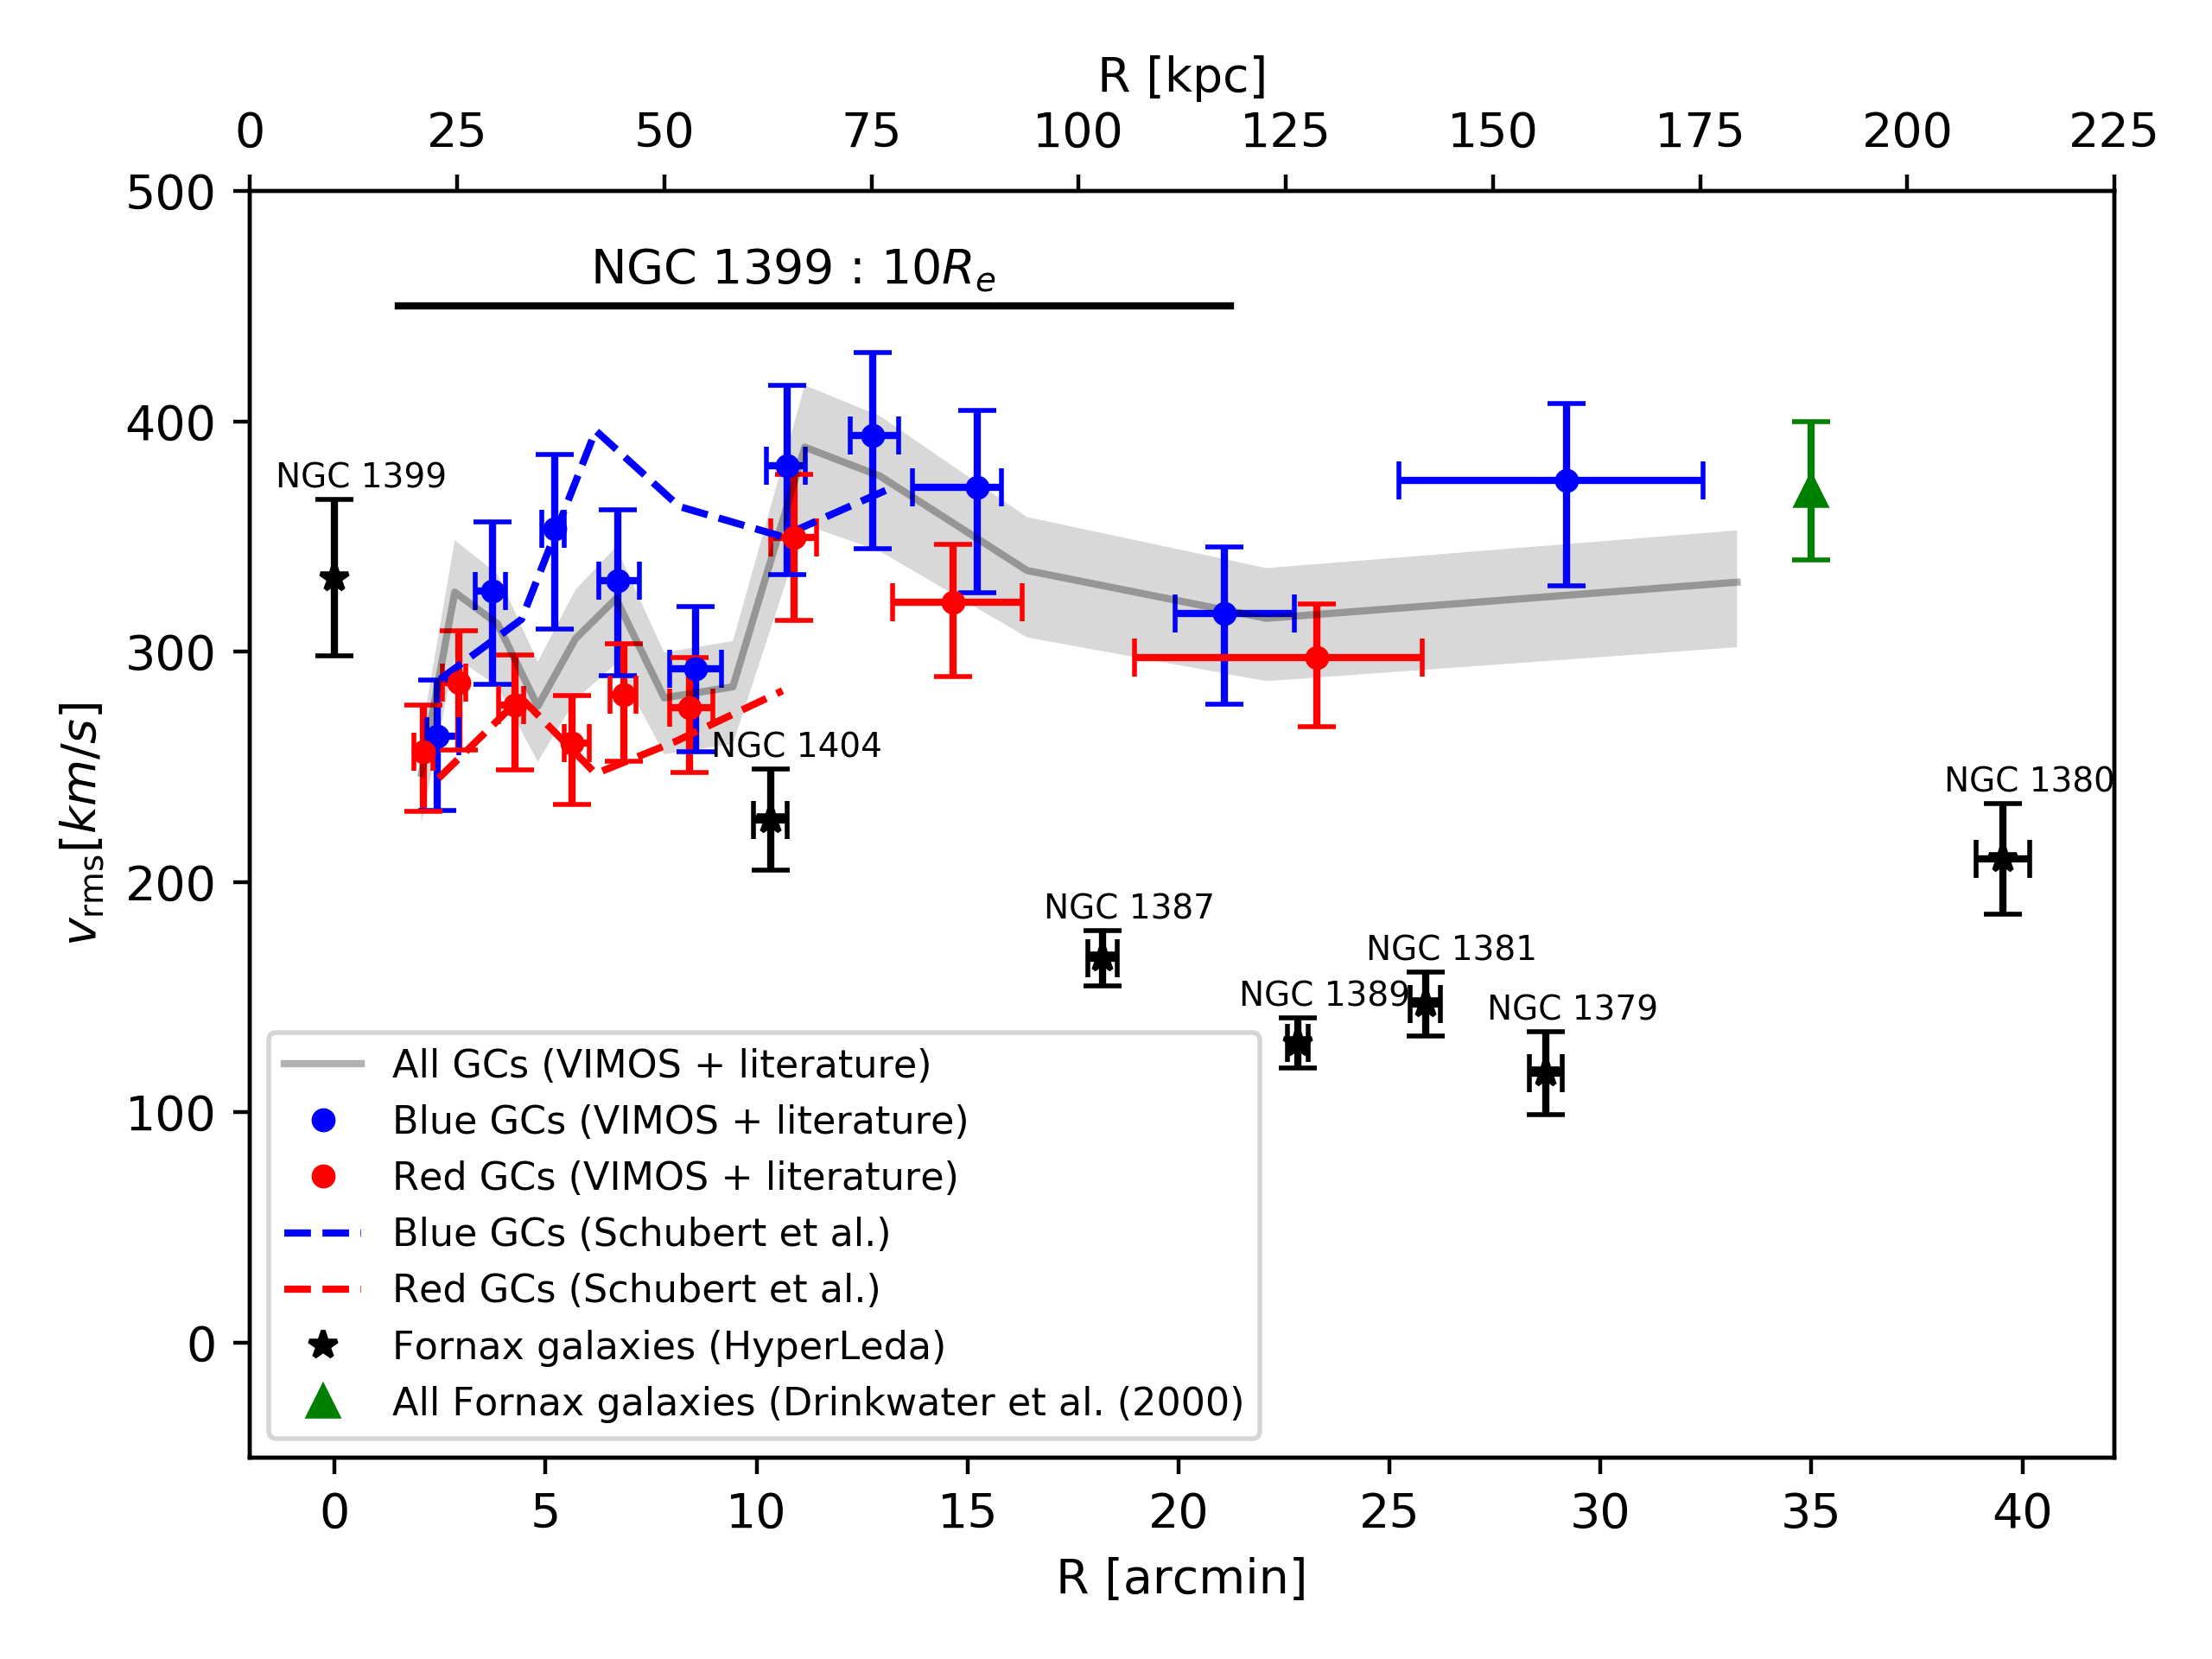
\includegraphics[width=\columnwidth]{figures/vrms.png} 
\caption{Root-mean-square velocity dispersion of NGC~1399 stellar system. The blue and red points represent the blue and red GCs/UCDs, respectively, whereas the full grey-line shows the full master catalogue of 1133 GCs/UCDs. Bins are of irregular size, reflected in the asymmetric radial error bars representing the 25-th and 75-th quantiles. The digitised $v_{\rm rms}$ profiles from \citet{Schuberth} are the blue and red dashed lines, without uncertainties for clarity. The central stellar velocity dispersion for the galaxies in the field are the black points, with the error bars on the x-axis representing one effective radius. The green triangle shows the innermost value of the velocity dispersion derived for Fornax galaxies by Drinkwater et al. (2001).}
%NRN: Aaaron asks about the green triangle: "say more about what radial range these dwarfs came from". But this is not about dwarf...it's all galaxies I don't know from where he thought so. I added the description of the green triangle
%NRN: Aaron asks to put error bars on N1399 as well (which does not make sense)...why don't we add a stellar profile instead? Chiara has it.
%NRN: I've made the figure 2 columns
\label{fig:vrms}
\end{figure*}

Figure \ref{fig:vrms} displays the $v_{\rm rms}$ profile for: i) our combined master catalogue of 1133 GCs and UCDs; ii) the GC catalogue of \citet{Schuberth}, iii) the central stars of galaxies surrounding NGC~1399; iv) all Fornax galaxies from \citet{Drinkwater00}. 

The master catalogue contains GCs and UCDs predominantly from NGC 1399, which is the largest and more massive system in the field dominating the total potential in the core of the cluster. Here, objects from other galaxies, embedded in the extended exponential halo around the galaxy (Iodice et al. 2016), in particular NGC 1404, NGC 1387, are likely to contaminate the kinematics of the central galaxies. However, looking at the $v_{\rm rms}$ profile of the total sample (shaded gray area) there is a steep rise in the profile around $R\sim10$ arcmin which marks a kinematical transition from a ``colder'' kinematical region ($\sim 50 kpc$) to a ``warmer'' one. In the outermost region, the $v_{\rm rms}$ profile flattens out to a value which is fairly consistent with the kinematics of the cluster galaxies (the green data point at $R\sim35’$ from \citealt{Drinkwater00}). This suggests that the GC kinematics at radii larger than 10 arcmin is ruled by the cluster potential. This feature demonstrates kinematically that the photometric transition radius between the bright central galaxy and the outer exponential halo at $R\sim10$ arcmin from \citet{Iodice16} represents the radius where we observe the emergence of an intracluster population of GCs. A similar conclusion is found for planetary nebulae by Spinello et al. (2018), and hence multiple lines of evidence are converging, for the first time, on the existence of a photometrically and kinematically distinct intracluster light population in the Fornax Cluster core.

When split in the red and blue subpopulations 
%NRN: Aaron asks to write how reds and blues are split
the GC sample shows some systematic differences. At all radii the $v_{\rm rms}$ profile of the red GCs is systematically smaller than the one of the blue GCs.  In the innermost regions at $R < 10$ arcmin they are consistent with the results from Schuberth et al. (2010a). In particular the blue GCs turn out to be the more extended population in radius, nicely connecting to the value of the cluster galaxy datapoint. The difference in normalisation between the two populations may be mainly driven from the different slopes of the two populations density profiles as measured, e.g., by Schuberth et al. (2010a, their Eq. 10 and 11 and Table 5). However, the difference between the measured slopes is so small that using Eq. 2 to 4 in Napolitano et al. (2014) to determine the expected change in the normalisation of the two profiles, we have found that for a $v_{\rm rms} \sim 300$ km s $^{-1}$ of the RGCs value the estimated BGCs value of $v_{\rm rms}$ is $\sim 308$ km s $^{-1}$, i.e. consistent with what we have measured for the Blue GC datapoint within the typical errors.

Finally, we report in the same Figure the central velocity dispersion values of the galaxies populating the same area occupied by the total GC catalog. The central value of NGC 1399 is consistent with the typical central rise of the velocity dispersion in the center of massive galaxies where the potential on the galaxy dominates. At larger distances one can expect that neighbouring might contaminate the overall GC kinematics. Especially in the outer regions, i.e. $R>10$ arcmin, assuming these regions are dominated by the cluster potential, the presence of GCs bound to the galaxies might alter the true  intracluster population. A detailed separation of the bound GC population from the true unbound (from any galaxy in the core) GCs will be addressed in a forthcoming paper. Here we just remark that the impact of the bound GC population must be limited because, roughly speaking, it should dilute the true dispersion by a quantity that it is about the difference in quadrature (at the most) of the true dispersion and that of the bound sample (i.e. assuming the central velocity dispersion of the galaxy). If so, then the dilution can be as large as 10-15$\%$, which is enough to explain the saddle in the  $v_{\rm rms}$ profile in the radius range $15<R<28$ arcmin corresponding to the bins overlapping with NGC~1387, NGC~1389, NGC~1381 and NGC~1379, while a similar correction for NGC~1404 at $R\sim10'$ would increase the intrinsic $v_{\rm rms}$ to $\sim400$ km s $^{-1}$, i.e. consistently with the peak value at $R\sim12'$.

In conclusion of this section, we can summarise the main finding of this paper in Figure 9, by saying that the unprecedented extension of the GC kinematics, combined with the literature data, has demonstrated the kinematical signature of a population of intracluster GCs, made of both red GCs and blue GCs. The two populations show $v_{\rm rms}$ profiles consistent with the dynamics of a common cluster potential and also consistent with the velocity dispersion of the innermost cluster galaxies in the Fornax cluster. 

Analogous signatures of intracluster stellar populations have been shown previously in the Virgo and Fornax clusters \citep[see e.g., ][]{Arnaboldi04, Longobardi15, Paolillo02} but the catalog presented here will offer a unique chance to perform a fully dynamical analysis of both the bound and unbound GC populations \citep{DAbrusco16}.

\section{Conclusions}
\label{sec:conclusions}
In this paper, we presented the results of the widest spectroscopic survey of GCs in the Fornax cluster ever realised, focusing on observations, data reduction and presentation of the final catalogue. This is the first work of a larger multi-instrument ptogram dubbed the Fornax Cluster VLT Spectroscopic Survey (FVSS), which, in sinergy with the ongoing Fornax Deep Survey (FDS), aims to study the formation, evolution and dynamics of galaxies and small stellar systems in the Fornax cluster.

Our analysis is based on observations with VST/OmegaCam for imaging and 25 VST/VIMOS masks for spectroscopic follow-up. Objects were pre-selected in multi-band imaging, supported also by the many spectroscopic catalogues already present for this region of the sky.  Approximately 4500 objects were observed. The total observation time was 37.5 hours, mostly in sub-arcsec seeing conditions. Data reduction was performed using the ESO VIMOS pipeline. Redshifts were extracted using iraf/fxcor, whereas the remaining data analysis was carried out using the python suite. Only the Calcium Triplet region was used for redshift estimation, but the quality of the fit was assessed using the full spectrum from 4800 to 10000 \AA\ .

After a visual inspection of candidate spectra, we compiled a consensus catalogue of 372 GCs, 15 UCDs (objects with $i \le 20.3$ mag) and 464 Galactic stars. Most GCs belong to the dominant galaxy NGC~1399, but we estimated that 30-40 objects might belong to NGC~1404, NGC~1380, and to other major galaxies in the observed field.

We have used the new complete catalog of GCs to derive the total  $v_{\rm rms}$ of the GC sample and also broken the sample in the red and blue subsamples.
%NRN: remember to explain how these are split 
We have demonstrated that all profiles show a similar signature at around $R\sim10’$ of a kinematical transition from a low $v_{\rm rms}$ regime to a higher one, with the former being consistent with the central velocity dispersion of NGC 1399 (the central cluster galaxy) and the latter being consistent with the velocity dispersion of the cluster galaxies. This demonstrates that at $R>10’$ both the GC populations feel strongly the cluster potential, rather than the more fable galaxy potential. Parallel to this paper we also performed a similar analysis where we present similar evidence based on kinematical distribution ot planetary nebulae (PNe) in the core of the cluster, up to 200kpc (Spiniello et al. 2018, submitted). PNe also show a rise in the velocity dispersion compatible with PNe tracing the potential of the cluster as a whole. A detailed kinematical characterization of these ICL populations, will be the topic of a forthcoming analysis. We just point out here that these kinematical evidences corroborate the photometric evidence, found in the deep galaxy photometry, of a transition radius between the bright central galaxy and the outer exponential halo at $R\sim10$ arcmin from Iodice et al. (2016) and show, from the dynamical point of view, the emergence of an intracluster population of GCs (as well as PNe) in the Fornax Cluster.


\bibliographystyle{mn2e}
\bibliography{ref3}
%NRN: in the biblio you have Schuberth twice!


\end{document}

>>>>>>> Romanosky_Hilker
